
%
\documentclass[runningheads]{llncs}
\usepackage{graphicx}
\usepackage{amsmath,amsfonts,amssymb}
\usepackage{array,booktabs}
\usepackage{parskip}
\usepackage{mathtools}
\usepackage{subfig}
%
\begin{document}
% title
\title{Nonlinear and Chaotic Pendulum Simulations Using Lagrangian Mechanics}
%\thanks{Supported by Mult x.} % if we want to thank someone/org.
%
% authors
\author{Timothy Holmes}
%
\authorrunning{Timothy Holmes}
% First names are abbreviated in the running head.
%
\institute{{DePaul University Department of Physics}}
%
\maketitle              % typeset the header of the contribution
%
\begin{abstract}
Lagrangian Mechanics is a simple way to solve complex classic problems. Lagrangian Mechanics can be used to find a systems equation of motion. A simple example of a trivial system is the simple pendulum, an easy system to model. Adding to this system another pendulum bob brings in a complex system that varies with the slightest initial conditions. Chaos theory in its simplest form is the concept of slight changes in the initial conditions leading to drastic differences in the system overtime. If the initial conditions of the system are known, the system can be integrated through infinite time to describe the overall system.
%
\keywords{Chaos Theory  \and Pendulum \and Lagrangian Mechanics.}
\end{abstract}
%
%
%
\section{Introduction}
\subsection{Chaos Theory}

Chaos theory arises in Lagrangian mechanics with the double pendulum, its extreme changes in motion based on ever so slight initial conditions show how different the out come will be. Chaos theory says that we are not able to predict exactly what the system will do. However, the system such as the double pendulum can be deterministic in such a computer model by integrating forward in time with infinite precision.  

\subsection{Computationally Modeling Nonlinear System}

The steps to solving a Lagrangian are general. In a high level overview of solving for the equations of motion for Lagrangian mechanics, the steps are in the following order. First you have to find the generalized coordinates $q$. Once found the kinetic and potential energies need to be accounted for. Finding the coordinate transformations from one coordinate system to another with the use of generalized coordinates and substituting the results into the energies will be enough for the Lagrangian. From there using the Euler-Lagrange equation will solve for the equations of motion for the given system. This is now enough information to set up a computational model. In essence, you can think of the modeling aspect as working backwards from the previous steps. Starting from the equations of motion, a function can be wrote to take the first derivative of the differential equation. A numerical method, such as runge kutta, is need to solve this differential equation. Once there is an output from the differential equation, the output can be applied back into the coordinate transformation. This is because it is easier to plot in Cartesian coordinates. After plotting the real analysis of the system begins. Changing initial parameters and plotting different generalized coordinates will tell a lot about the system at hand.


\section{Lagrangian Mechanics and the Pendulum}
\subsection{The Simple Pendulum}

\subsubsection{Finding the Equations Of Motion.}

The most simplistic physical system is the simple pendulum. Understanding the simple pendulum and building from it will help later on to derive the double pendulum, which is only slightly more advanced than the simple pendulum. Furthermore, understanding the simple pendulums motion will make it easier to understand the motion of the harmonically driven pendulum and the rotational pendulum. \\

Starting to build the problem the first thing that can be found for the simple pendulum is the kinetic energy term $T$. The pendulum bob is free it move in the $x$ and $y$ coordinates. Therefore, the kinetic energy for this system can be described as $T = 1/2m(\dot{x^2} + \dot{y^2})$. This system only has one potential energy term that is affected by gravity. The potential energy for this system is $V = mgy$. Using generalized coordinated, a coordinate transformation is performed to make the problem easier to solve. Setting the coordinates 


\begin{align*}
 x &= \ell sin(\theta) & y &= -\ell cos(\theta).
\end{align*}

The $x$ coordinate transformation is positive and the $y$ coordinate transformation is negative because we set the origin is up and to the left of the pendulum bob. Taking the time derivative and squaring the new coordinates results in

\begin{align*}
 \dot{x} &= \ell cos(\theta)\dot{\theta} & \dot{y} &= -\ell sin(\theta)\dot{\theta} \\
 \dot{x}^2 &= \ell^{2}cos^{2}(\theta)\dot{\theta}^{2} & \dot{y}^2 &= \ell^{2}sin^{2}(\theta)\dot{\theta}^{2}.
\end{align*}

Knowing that the Lagrangian is kinetic energy minus potential energy $L = T - V$ and entering the transformed coordinates into $T$, $V$, the Lagrangian becomes,

\begin{equation}
    L = \frac{1}{2}m(\ell^{2}cos^{2}(\theta)\dot{\theta}^{2} + \ell^{2}sin^2(\theta)\dot{\theta}^{2}) + mg\ell cos(\theta).
\end{equation}

Factoring out $\ell^{2}$ and $\dot{\theta}^{2}$ terms from the kinetic energy portion of the Lagrangian reduces the equation to $1/2m(\ell^{2}\dot{\theta}^{2}(sin^{2}(\theta) + cos^{2}(\theta)))$. Using the trigonometric identity $sin^{2}(\theta) + cos^{2}(\theta) = 1$. The Lagrangian reduces to

\begin{equation}
    L = \frac{1}{2}m\ell^{2}\dot{\theta}^{2} + mg\ell cos(\theta).
\end{equation}

To find the equation of motion the Euler-Lagrangian equation is used

\begin{equation}
    \frac{d}{dt}\frac{\partial L}{\partial \dot{\theta}} - \frac{\partial L}{\partial \theta} = 0.
\end{equation}


Leaving a few differentiating steps and reducing out the final equation of motion that describes the simple pendulum is

\begin{equation}
    \ddot{\theta} = -\frac{g}{\ell}sin(\theta).
\end{equation}

Now that the equation of motion is defined the simulation can start.

\subsubsection{The Modeled Results.}

\begin{figure}%
    \centerinR
    \subfloat[Simple pendulum bob path.]{{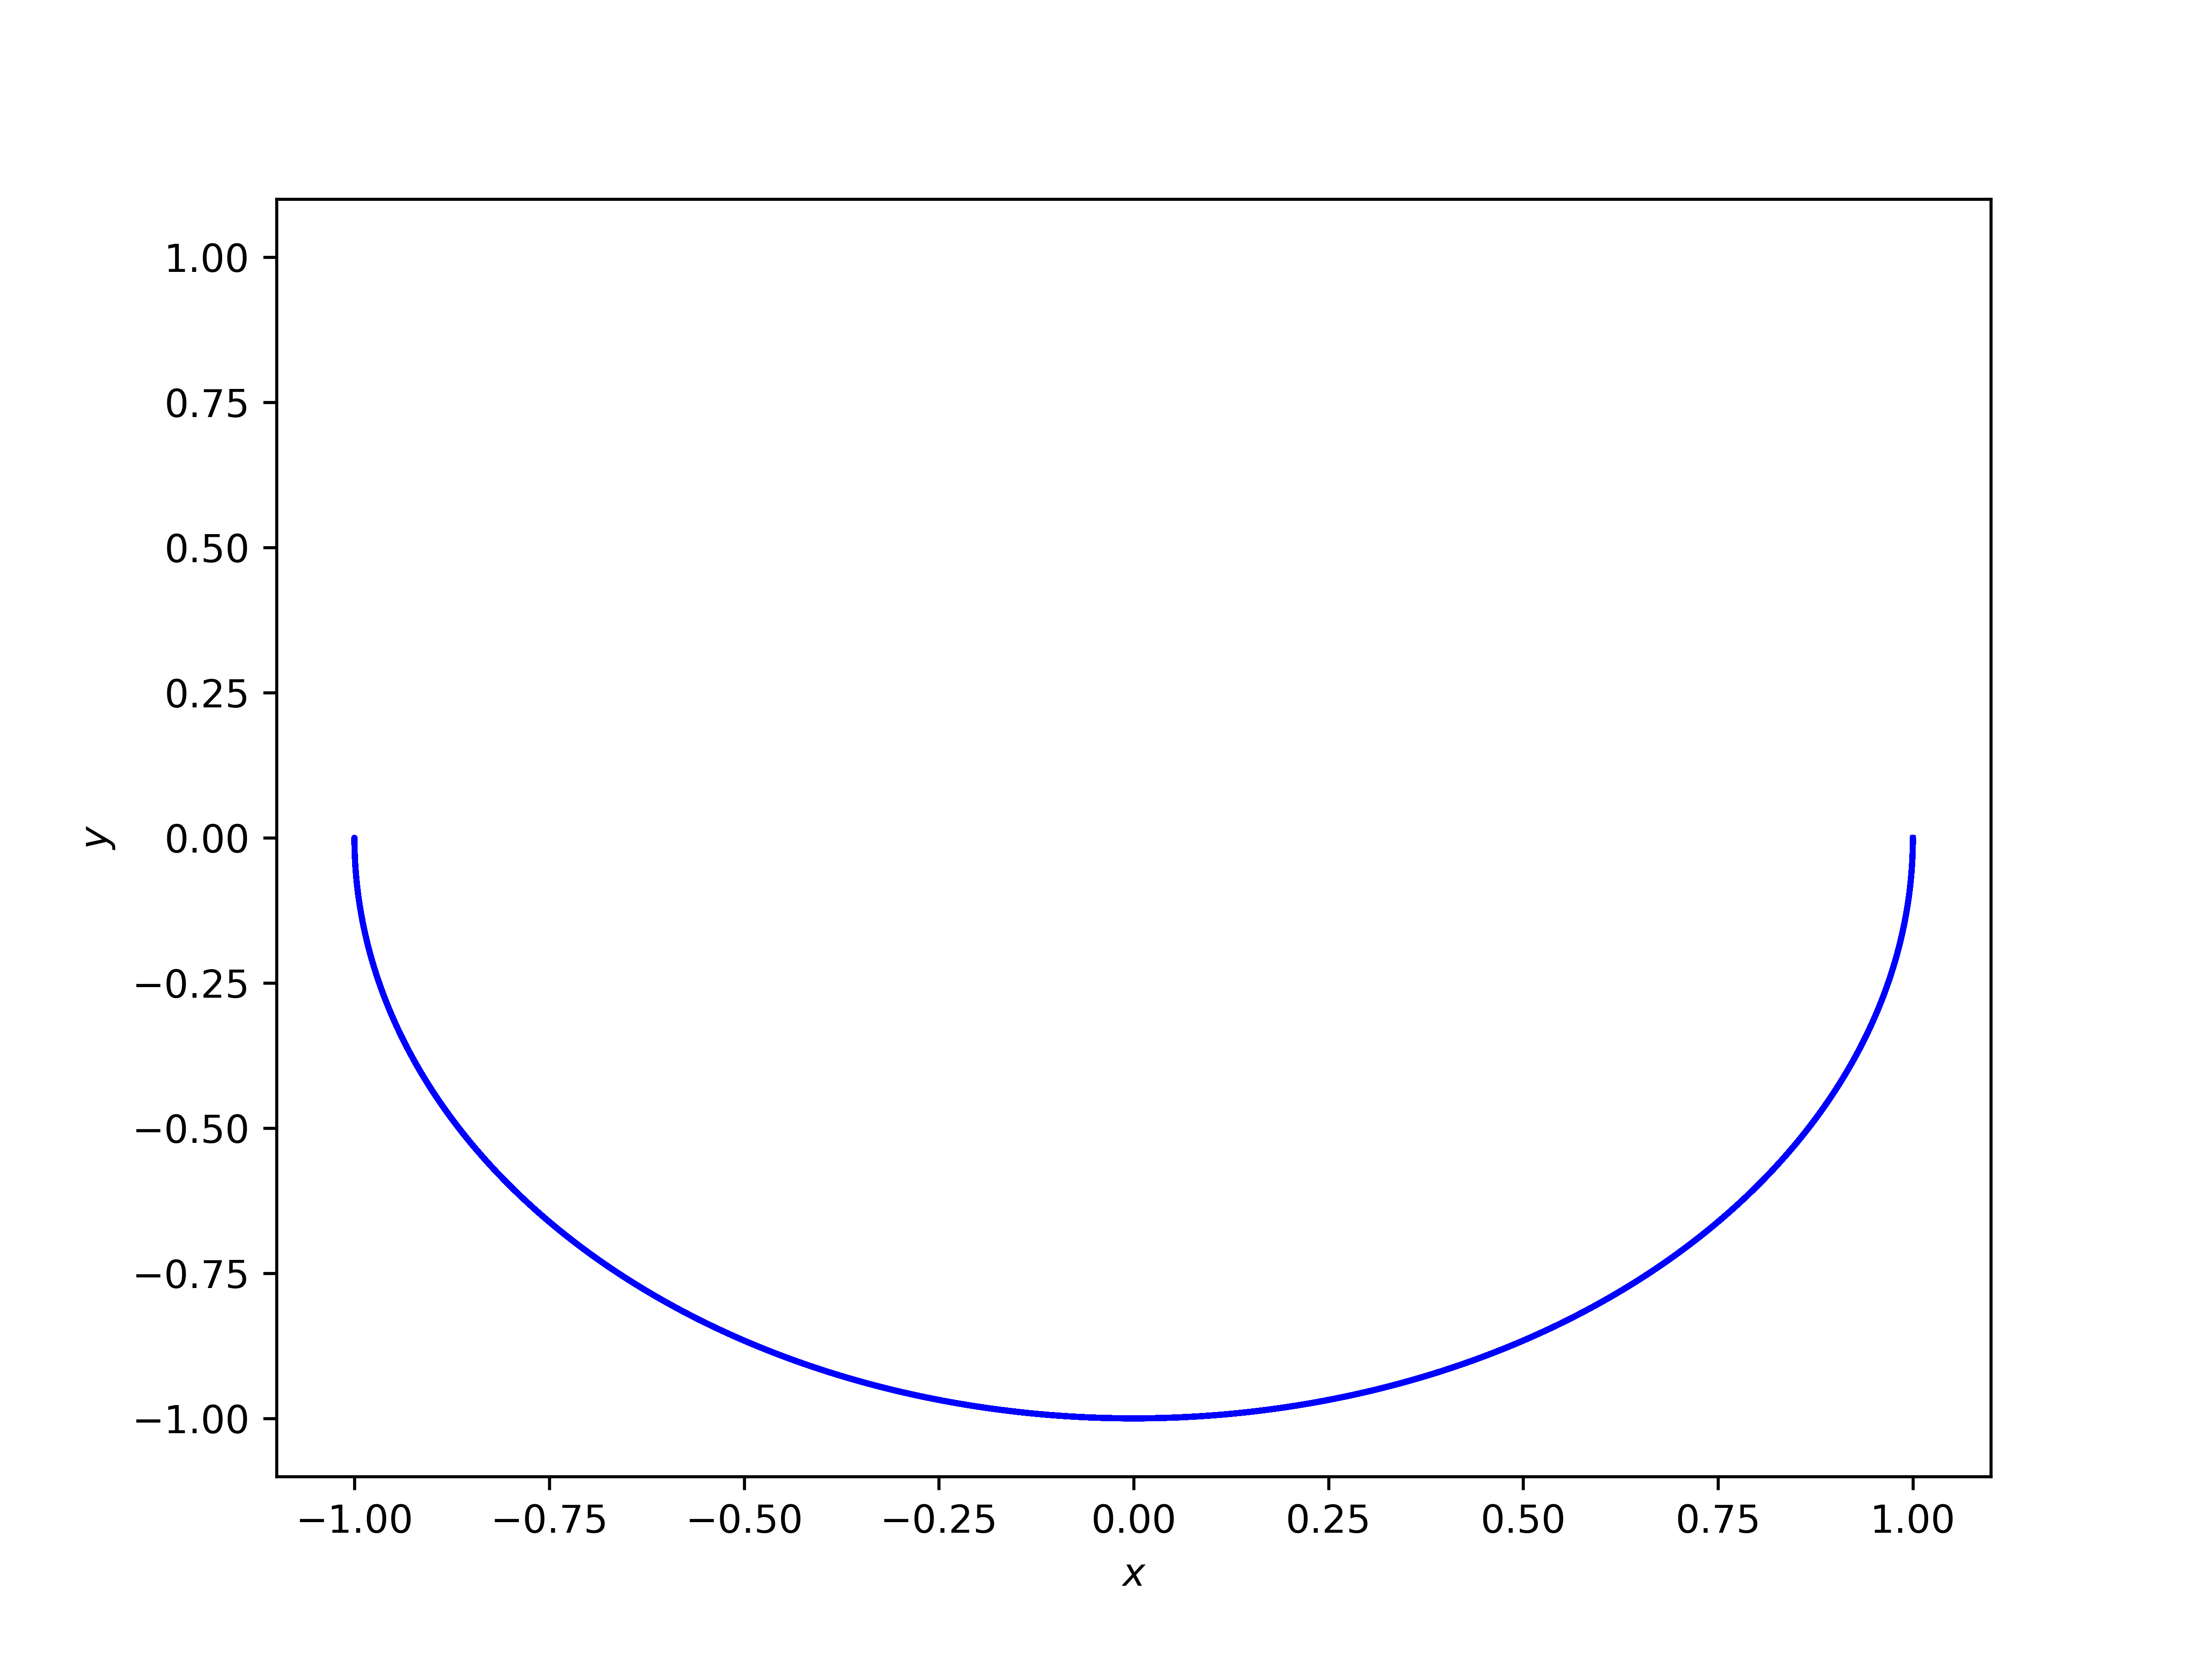
\includegraphics[width=5.5cm]{img/simple_pendulum_path.png} }}%
    \qquad
    \subfloat[Simple pendulum angle over time.]{{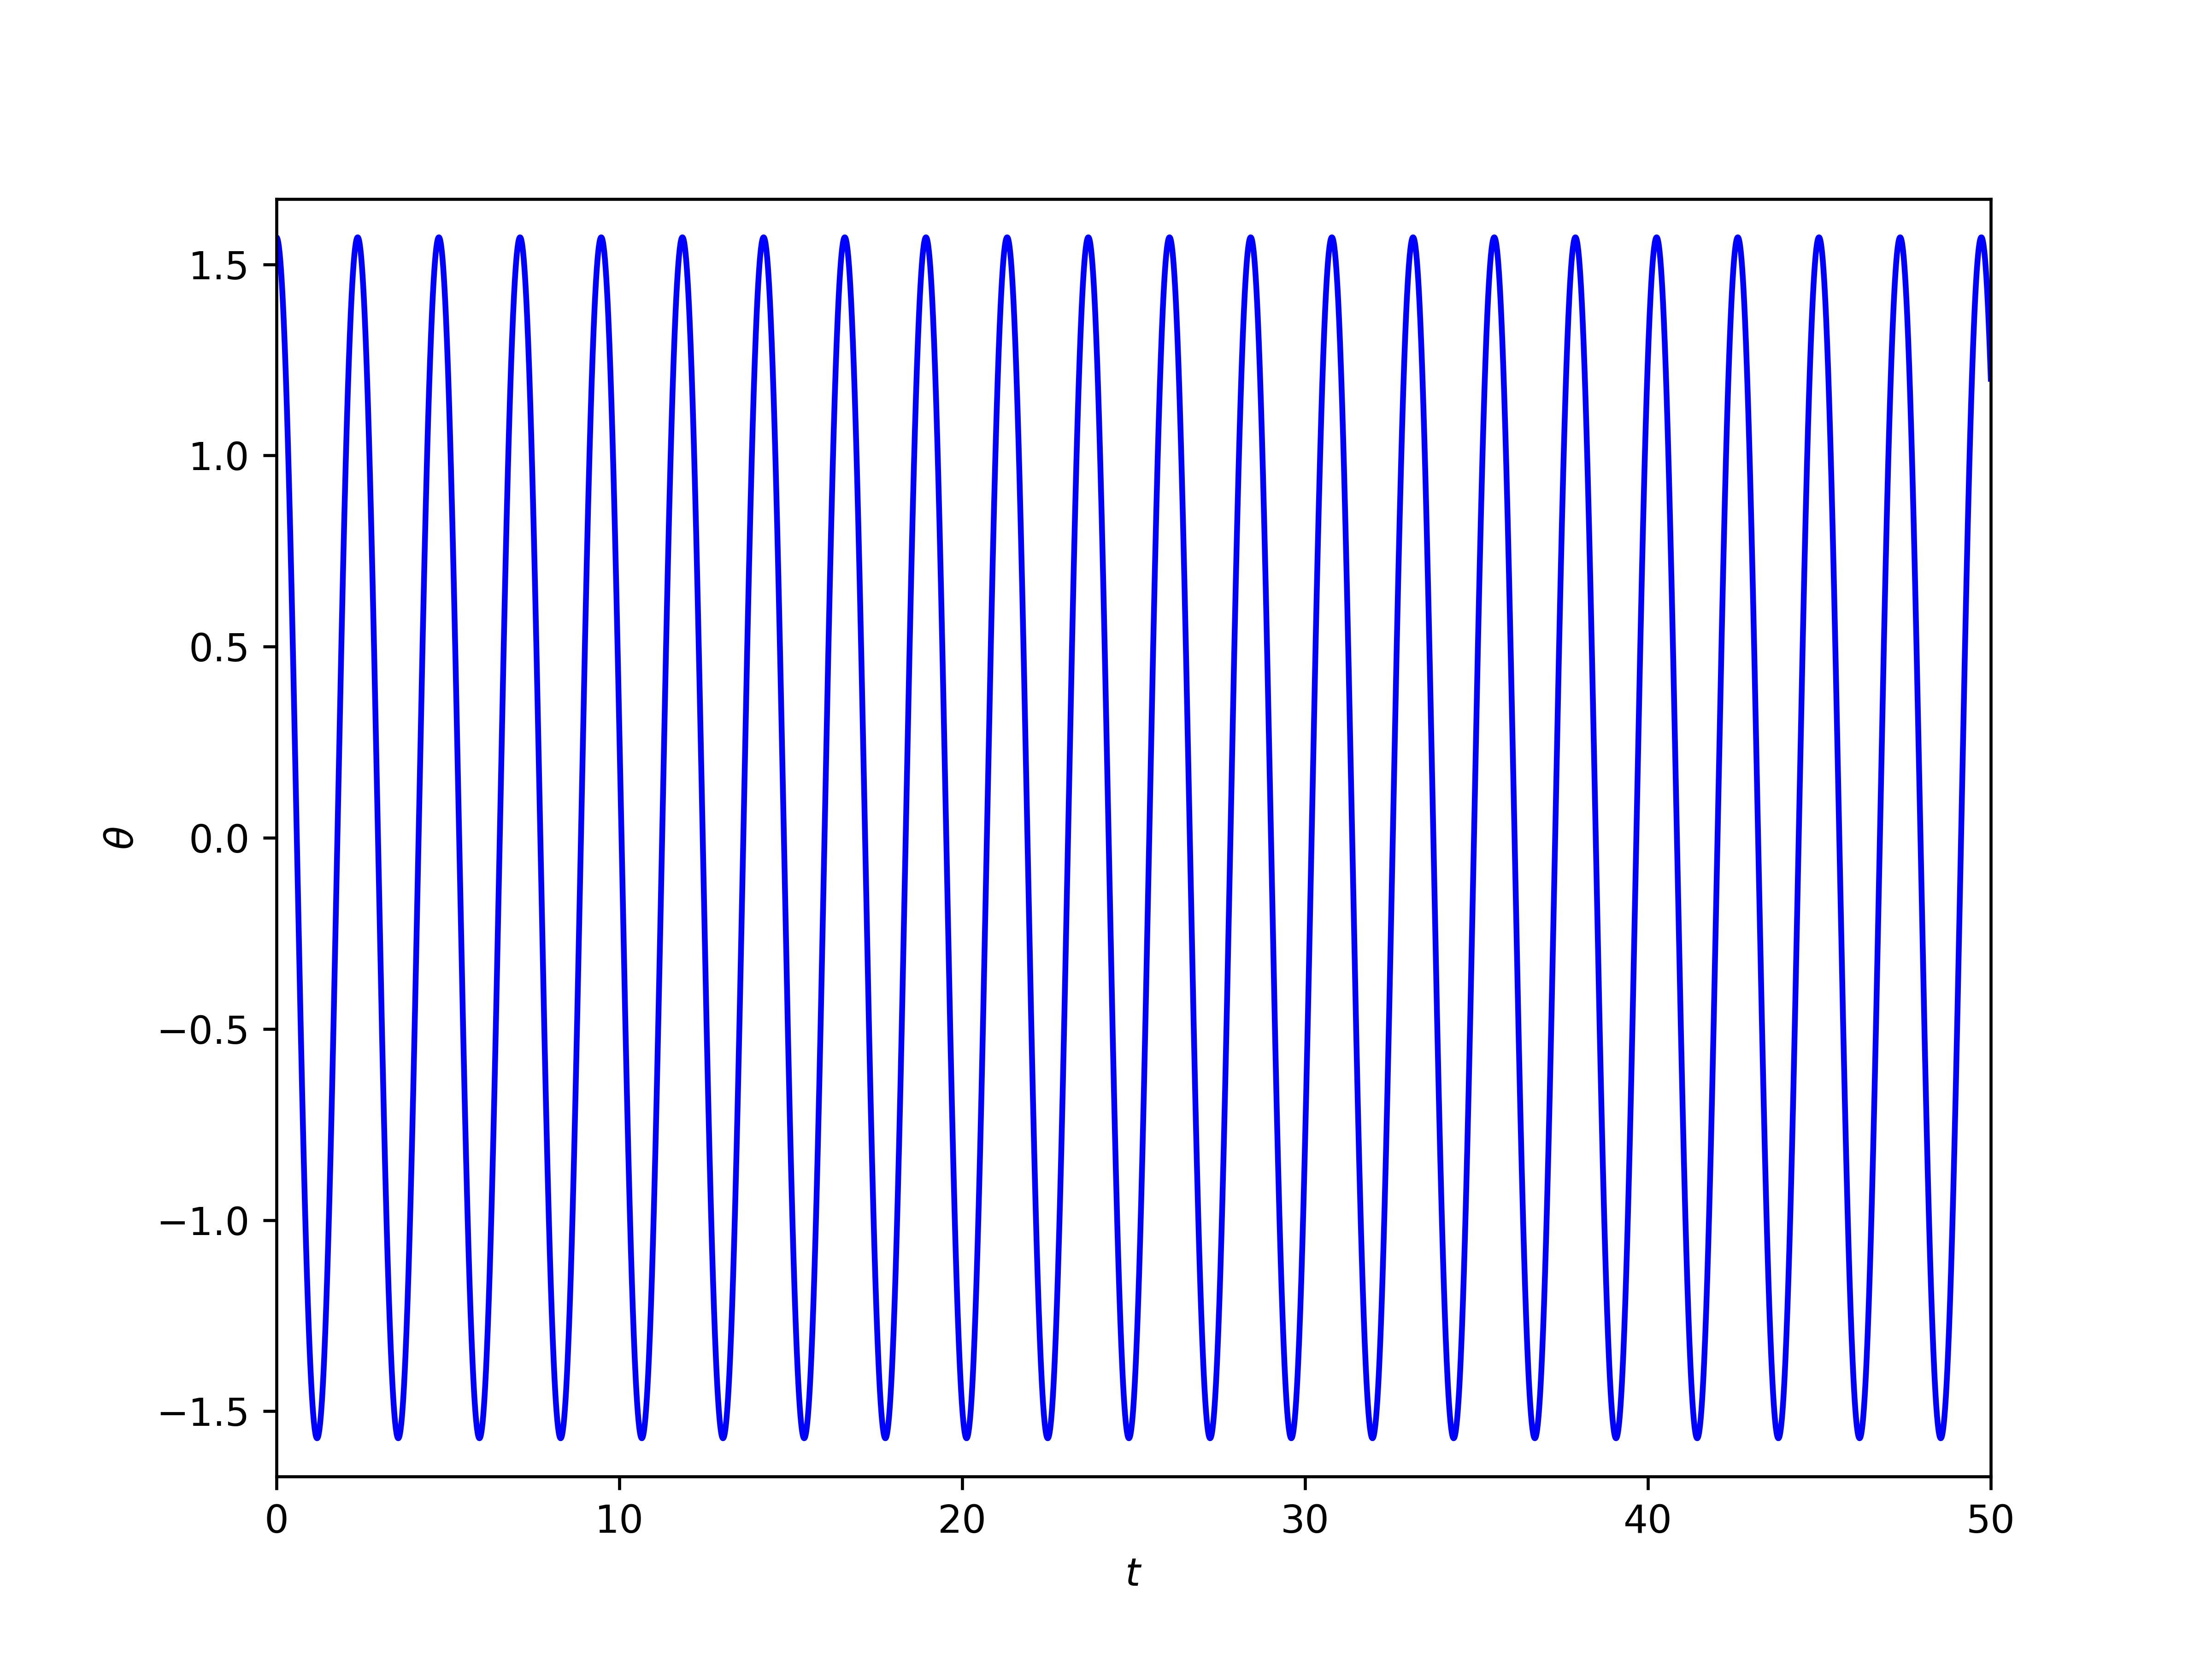
\includegraphics[width=5.5cm]{img/simple_pendulum_angle.png} }}%
    \caption{The simple pendulum model}%
    \label{fig:example}%
\end{figure}

Above in Fig. 1 shows graphs pulled from the simple pendulum model. Sub-figure (a) shows the path the pendulum's bob moves. As we can see the initial conditions were set up in a way to allow the pendulums rod is parallel with the x-axis. The path of the bob is then just a half a circle, it is clear from figure one that the pendulums bob can only move around this circle with radius $\ell$, the length of the rod. If the initial conditions were set up in a way that the bob started in the positive y-axis at $x = 0$, the path of the pendulum would be a complete circle. \\

In Sub-figure (b) a sinusoidal pattern is plotted, that is the plot is the pendulums angle over time. This should be expected since the equation of motion has a $sin$ term in it. Therefore, the simple pendulum moves with sinusoidal motion. \\

\subsubsection{Frequency in The Simple Pendulum.}

Another possibility of computationally modelling these systems is making all aspects of plotting easier. The frequency vs amplitude plot may become interesting when a force is involved or a more complex system is modeled. In the case of the simple pendulum in its most basic form, nothing of interest will come up. If we take the equation of motion component of a simple harmonic motion, $Acos(ft)$. Therefore, the frequency of the simple pendulum is $\omega^{2} = g\l$ or

$$
\omega = \sqrt{\frac{g}{l}}.
$$

knowing the frequency now the period happens every full cycle which is every $2 \pi$. The period of the simple pendulum is simply 

$$
T = 2\pi \sqrt{\frac{g}{l}}.
$$

Computationally the simple pendulum gets even more interesting if you add in a dampening term that is able to over damp or over damp the system. For the sake of simplicity, this can be shown more complex systems where the analysis is more involved but shows more interesting results.

%%%%%%%%%%%%%%%%%%%%%%%%%%%%%%%%%%%%%%%%%%%%%%%%%%%%%%%%%%%%%%%%%%%%
%
%       Chaos with forces
%
%%%%%%%%%%%%%%%%%%%%%%%%%%%%%%%%%%%%%%%%%%%%%%%%%%%%%%%%%%%%%%%%%%%%

\section{Computation of Non-Linear Systems with Forces}
\subsection{The Harmonically Driven Simple Pendulum}

\subsubsection{Finding the Equations of Motion.}

Similar to the simple pendulum, a pendulum that is driven with harmonic motion from the pendulum connecting point changes our expectation of the equation of motion. For a pendulum with some force the coordinate transformations from a simple pendulum will change. The new coordinates of the system will becomes

\begin{align*}
x &= \ell sin(\theta) + Dsin(\omega t + \phi) & y = \ell cos(\theta) \\
\dot{x} &= \ell cos(\theta) \dot{\theta} + D\omega cos(\omega t + \phi) & \dot{y} = -\ell sin(\theta) \dot{\theta}. \\
\end{align*}

The difference in this coordinate transformation compared to the simple pendulum is that the x term now has an extra $D sin(\omega t = \phi)$. This is the extra term that is responsible for the external for that drives the pendulum. Also find the Lagrangian these coordinates also need to be squared. Expanding the squared terms results in

\begin{align*}
\dot{x}^{2} &= \ell^{2}\dot{\theta}^{2} cos^{2}(\theta) + D^{2}\omega^{2}cos^{2}(\omega t + \phi) + 2\ell D\omega \dot{\theta}cos(\theta)cos(\omega t + \phi) \\
\dot{y}^{2} &= \ell^{2}\dot{\theta}^{2}sin^{2}(\theta).
\end{align*}

The new coordinates are now ready to be substitute into the kinetic energy and potential energy. The pendulum is free to move in both the x-axis and y-axis. Therefore the kinetic energy for this system is 

$$
T = \frac{1}{2}m(\dot{x}^{2} + \dot{y}^{2}).
$$

\noindent

Furthermore, the potential energy for the system is just dependent on the gravitational potential. This potential energy is 

$$
V = mgy.
$$


\noindent
The Lagrangian in its reduced form for this system is then just simply 

\begin{align*}
L &= \frac{1}{2}m(\ell^{2}\dot{\theta}^{2} + D^{2}\omega^{2}cos^{2}(\omega t + \phi) + 2\ell D \omega \dot{\theta} cos(\omega t + \phi)cos(\theta)) + mg\ell cos(\theta)
\end{align*}

Since the Lagrangian has been found for the system the equation of motion can be found using the Euler-Lagrangian Equation. Solving for the equations of motion 

\begin{align*}
&\frac{d}{dt} \frac{\partial L}{\partial \dot{\theta}} = m\ell^{2} \ddot{\theta} - m\ell D\omega^{2} sin(\omega t + \phi)\\
&\frac{\partial L}{\partial \theta} =  - mg\ell sin(\theta).\\
\end{align*}

The reduced equation of motion for this system is 

$$
\ddot{\theta} + \frac{g}{\ell} sin(\theta) = \frac{D}{\ell}\omega^{2} sin(\omega t + \phi).
$$

\subsubsection{The Modeled Results.}

\begin{figure}%
    \centering
    \subfloat[Model of the harmonic pendulum.]{{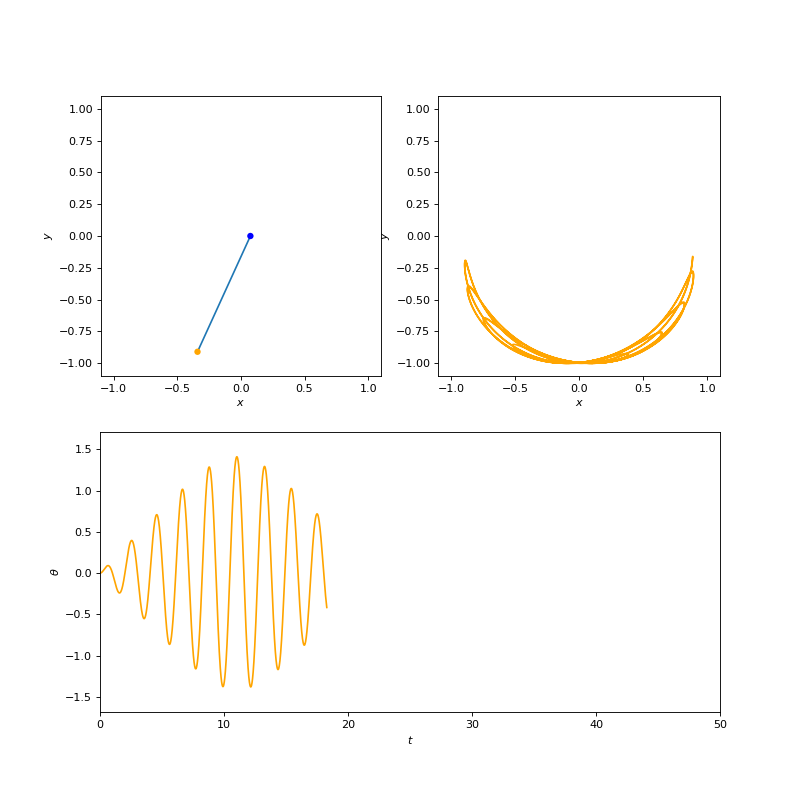
\includegraphics[width=5.5cm]{img/harmonic_pen.png} }}%
\end{figure}

The figure above shows an example of the model running. There is not too much different in relation to the simple pendulum other than the fact that this model has an external force driving it. $\omega_0$ can be found for this model just like with the simple pendulum. It turns out the it is the same as it was for the simple pendulum. The length used was 1 meter and the gravitational constant was 9.81. This means that $\omega_0 = 3.13$. When the parameter for $\omega$ was set to this value the $\theta$ vs time graph has a beating affect to it. This is something that can not be seen in the simple pendulum model and is dependant on the fore driving it for this effect to happen.

%%%%%%%%%%%%%%%%%%%%%%%%%%%%%%%%%%%%%%%%%%%%%%%%%%%%%%%%%%%%%%%%%%%%
%
%       Rotational Pendulum
%
%%%%%%%%%%%%%%%%%%%%%%%%%%%%%%%%%%%%%%%%%%%%%%%%%%%%%%%%%%%%%%%%%%%%


\subsection{The Rotational Simple Pendulum}

\subsubsection{Finding the Equations of Motion.}

Much like the harmonically driven pendulum, the rotational pendulum also has a force applied to it that allows it to travel around a fix circle of radius R. Therefore, the coordinate transformation is closely related. The coordinate transformation for a rotational pendulum is

\begin{align*}
x &= \ell sin\theta + Rsin(\omega t) & y = - \ell cos\theta + Rcos(\omega t) \\
\dot{x} &= \ell cos\theta \dot{\theta} - R\omega cos(\omega t) & \dot{y} = \ell sin\theta \dot{\theta} - R\omega sin(\omega t). \\
\end{align*}

Again, this looks exactly like the simple pendulum. However, in the case of the $x$ coordinate an additional $Rsin(\omega t)$ is added on and in the case of the $y$ coordinate an additional $Rcos(\omega t)$. All these additional terms are describing are where the attachment point of the pendulum is on the circle at time $t$. Now, the kinetic energy need the time derivative coordinates expanded as squred terms, these terms are as follow

\begin{align*}
\dot{x}^{2} &= \ell^{2}cos^{2}(\theta) \dot{\theta}^{2} + R^{2}\omega^{2}cos^{2}(\omega t) + 2\ell \dot{\theta}R\omega cos(\theta)cos(\omega t) \\
\dot{y}^{2} &= \ell^{2}sin^{2}(\theta) \dot{\theta}^{2} + R^{2}\omega^{2}sin^{2}(\omega t) + 2\ell \dot{\theta}R\omega sin(\theta)sin(\omega t).
\end{align*}

By now it may have become apparent that the kinetic and potential energy terms are the same for all pendulum systems. In fact, this is also true for the double pendulum later on but will have two kinetic and two potential energy terms. The reduced Lagrangian for this system is becomes

\begin{align*}
L &= \frac{1}{2}m(\ell^{2} \dot{\theta}^{2} + 2\ell \dot{\theta}R\omega(cos(\theta + \omega t))) + mg(\ell cos(\theta)).
\end{align*}


Now that we have the transformed Lagrangian the equations of motion can be found using the Euler-Lagrange equation and since there is only one coordinate we only have to find $\theta$. Therefore we have,


\begin{align*}
&\frac{d}{dt} \frac{\partial L}{\partial \dot{\theta}} = ml^{2}\ddot{\theta} -ml R\omega^{2}sin(\theta + \omega t)\\
& \frac{\partial L}{\partial \theta} =  mglsin(\theta). \\
\end{align*}

\noindent
The final equation becomes

$$
\ddot{\theta} + \frac{g}{l}sin(\theta) = \frac{R}{l}\omega^{2}sin(\theta + \omega t).
$$

\subsubsection{The Modeled Results.}

Nothing of interest came from this model. This model is very similar to the previous harmonically driven model. This should be expected. While it is still interesting to try this out and see what happens, much of the same can be described for this one.


%%%%%%%%%%%%%%%%%%%%%%%%%%%%%%%%%%%%%%%%%%%%%%%%%%%%%%%%%%%%%%%%%%%%
%
%       Double Pendulum
%
%%%%%%%%%%%%%%%%%%%%%%%%%%%%%%%%%%%%%%%%%%%%%%%%%%%%%%%%%%%%%%%%%%%%
\subsection{The Double Pendulum}



\subsubsection{Finding the Equations of Motion.}

A double pendulum is closely related to how a simple pendulum works. Instead of one pendulum bob, there are now two pendulum bobs that have to be taken into account. This introduces a new $\theta$, $\ell$, and $m$ term. Therefore, for a double pendulum there is $\theta_{1}$, $\theta_{2}$, $\ell_{1}$, $\ell_{2}$, $m_{1}$, and $m_{2}$. Based on the first bobs position and the second bobs position there are two coordinates to keep track of them; $x_{1}$, $y_{1}$, $x_{2}$, and $y_{2}$. \\

Based on what was described above and what was seen with the simple pendulum, a coordinate transformation is need. As in the simple pendulum we will assume that the pendulum bobs are in the positive $x$ direction and the negative $y$ direction from the origin. Therefore, the coordinate transformations are

\begin{align*}
 x_{1} &= \ell_{1} sin(\theta_{1}) & y_{1} &= -\ell_{1} cos(\theta_{1}) \\
 x_{2} &= \ell_{1} sin(\theta_{1}) + \ell_{2} sin(\theta_{2}) & y_{2} &= -\ell_{1} cos(\theta_{1}) -\ell_{2} cos(\theta_{2}).
\end{align*}

The kinetic energy portion of the system are created in terms of velocity. The equations above need a time derivative that results in

\begin{align*}
 \dot{x}_{1} &= \ell_{1} cos(\theta_{1})\dot{\theta_{1}} & \dot{y}_{1} &= \ell_{1} sin(\theta_{1})\dot{\theta_{1}} \\
 \dot{x}_{2} &= \ell_{1} cos(\theta_{1})\dot{\theta_{1}} + \ell_{2} cos(\theta_{2})\dot{\theta_{2}} & \dot{y}_{2} &= \ell_{1} sin(\theta_{1})\dot{\theta_{1}} + \ell_{2} sin(\theta_{2})\dot{\theta_{2}}.
\end{align*}

Finally, the terms above have to be squared to be entered in the kinetic energy part. When squared the $\dot{x}$ and $\dot{y}$ terms are

\begin{align*}
 \dot{x}_{1}^{2} &= \ell_{1}^{2} cos^{2}(\theta_{1})\dot{\theta_{1}}^{2} \\
 \dot{y}_{1}^{2} &= \ell_{1}^{2} sin^{2}(\theta_{1})\dot{\theta_{1}} ^{2}\\ 
 \dot{x}_{2}^{2} &= \ell_{2}^{2}cos^{2}(\theta_{2})\dot{\theta_{2}}^{2} + \ell_{1}^{2}cos^{2}(\theta_{1})\dot{\theta_{1}}^{2} + 2\ell_{1}\ell_{2}cos(\theta_{1})cos(\theta_{2})\dot{\theta_{1}}\dot{\theta_{2}} \\
 \dot{y}_{2}^{2} &= \ell_{2}^{2}sin^{2}(\theta_{2})\dot{\theta_{2}}^{2} + \ell_{1}^{2}sin^{2}(\theta_{1})\dot{\theta_{1}}^{2} + 2\ell_{1}\ell_{2}sin(\theta_{1})sin(\theta_{2})\dot{\theta_{1}}\dot{\theta_{2}} \\ 
\end{align*}

There are now two different objects connected affecting one another in this system. This leaves the kinetic energy term $T$ as $T = 1/2m_{1}(\dot{x_{1}^{2}} + \dot{y_{1}^{2}}) + 1/2m_{2}(\dot{x_{2}^{2}} + \dot{y_{2}^{2}})$. This is again similar to the simple pendulum but now there is an additive term that represents the second pendulum bob. The potential energy term is only affected by gravity. The potential energy for this system is $V = m_{1}gy_{1} + m_{2}gy_{2}$. As shown before the additive term just counts for the second pendulum bob. This begins a clear pattern that can be seen for n number of pendulum bobs. The Lagrangian is described as $L = T - V$, the Lagrangian equation becomes 

\begin{equation}
    L = \frac{1}{2}m_{1}(\dot{x_{1}^{2}} + \dot{y_{1}^{2}}) + \frac{1}{2}m_{2}(\dot{x_{2}^{2}} + \dot{y_{2}^{2}}) + m_{1}gy_{1} + m_{2}gy_{2}
\end{equation}

Before entering all of the coordinate transformations some reducing can be done so that the equation isn't as long. There are two trigonometric identities that simplify this equation nicely. The first is $sin(x) + cos(x) = 1$. The other is the double angle identity which is $sin(x)sin(y) + cos(x)cos(y) = cos(x - y)$. After taking this into account the Lagrangian is 

\begin{multline}
    L = \frac{1}{2}(m_{1} + m_{2}) \ell_{1}^{2}\dot{\theta_{1}}^{2} + \frac{1}{2}m_{2}\ell_{2}^{2}\dot{\theta_{2}}^{2} + m_{2}\ell_{1}\ell_{2}  \dot{\theta_{1}}\dot{\theta_{2}}cos(\theta_{1} - \theta_{2})\\ + (m_1 + m_2)g\ell_{1}cos(\theta_{1}) + m_{2}g\ell_{2}cos(\theta_{2}).
\end{multline}

To find the equations of motion the Euler-Lagrangian is used. The Euler Lagrangian was given in equation (3). Since there are two theta terms there will be two different equations of motion that will describe the system. After taking partial derivatives, time derivatives, and using the method of substitution the two equations of motion are 

\begin{multline}
    \ddot{\theta_{1}} = \frac{\splitfrac{(m_{2}gsin(\theta_{2})cos(\theta_{1} - \theta_{2}) - m_{2}sin(\theta_{1} -  \theta_{2}) (\ell_{1}\dot{\theta_{1}}^{2}cos(\theta_{1}- \theta{2}) \ell_{2}\dot{\theta_{2}}^{2})}{  - (m_{1} + m_{2})gsin(\theta_{1}))}}{\ell_{1}(m_{1} + m_{2}sin^{2}(\theta_{1} - \theta_{2}))}
\end{multline}

and

\begin{equation}
   \ddot{\theta_{2}} = \frac{\splitfrac{(m_{1} + m_{2})(\ell_{1}\dot{\theta_{1}}^{2}sin(\theta_{1} - \theta_{2}) - gsin(\theta_{2}) + gsin(\theta_{1})cos(\theta_{1} - \theta_{2}))}{  + m_{2}\ell_{2}\dot{\theta_{2}}^{2}sin(\theta_{1} - \theta_{2})cos(\theta_{1} - \theta_{2})}}{\ell_{2}(m_{1} + m_{2}sin^{2}(\theta_{1} - \theta_{2}))}
\end{equation}

\subsubsection{The Modeled Results.}

With the equations of motion defined for a double pendulum, there is now a chance to simulate what this system is doing. By just adding one bob that depends on the other the system gets very chaotic and has more freedom then being limited to moving around a circle. If we start the double pendulum with minor initial conditions, that is start it on with a small angle, a sinusoidal pattern is found. The Figure below shows the first instance of this.

\begin{figure}%
    \centering
    \subfloat[Double pendulum bob path.]{{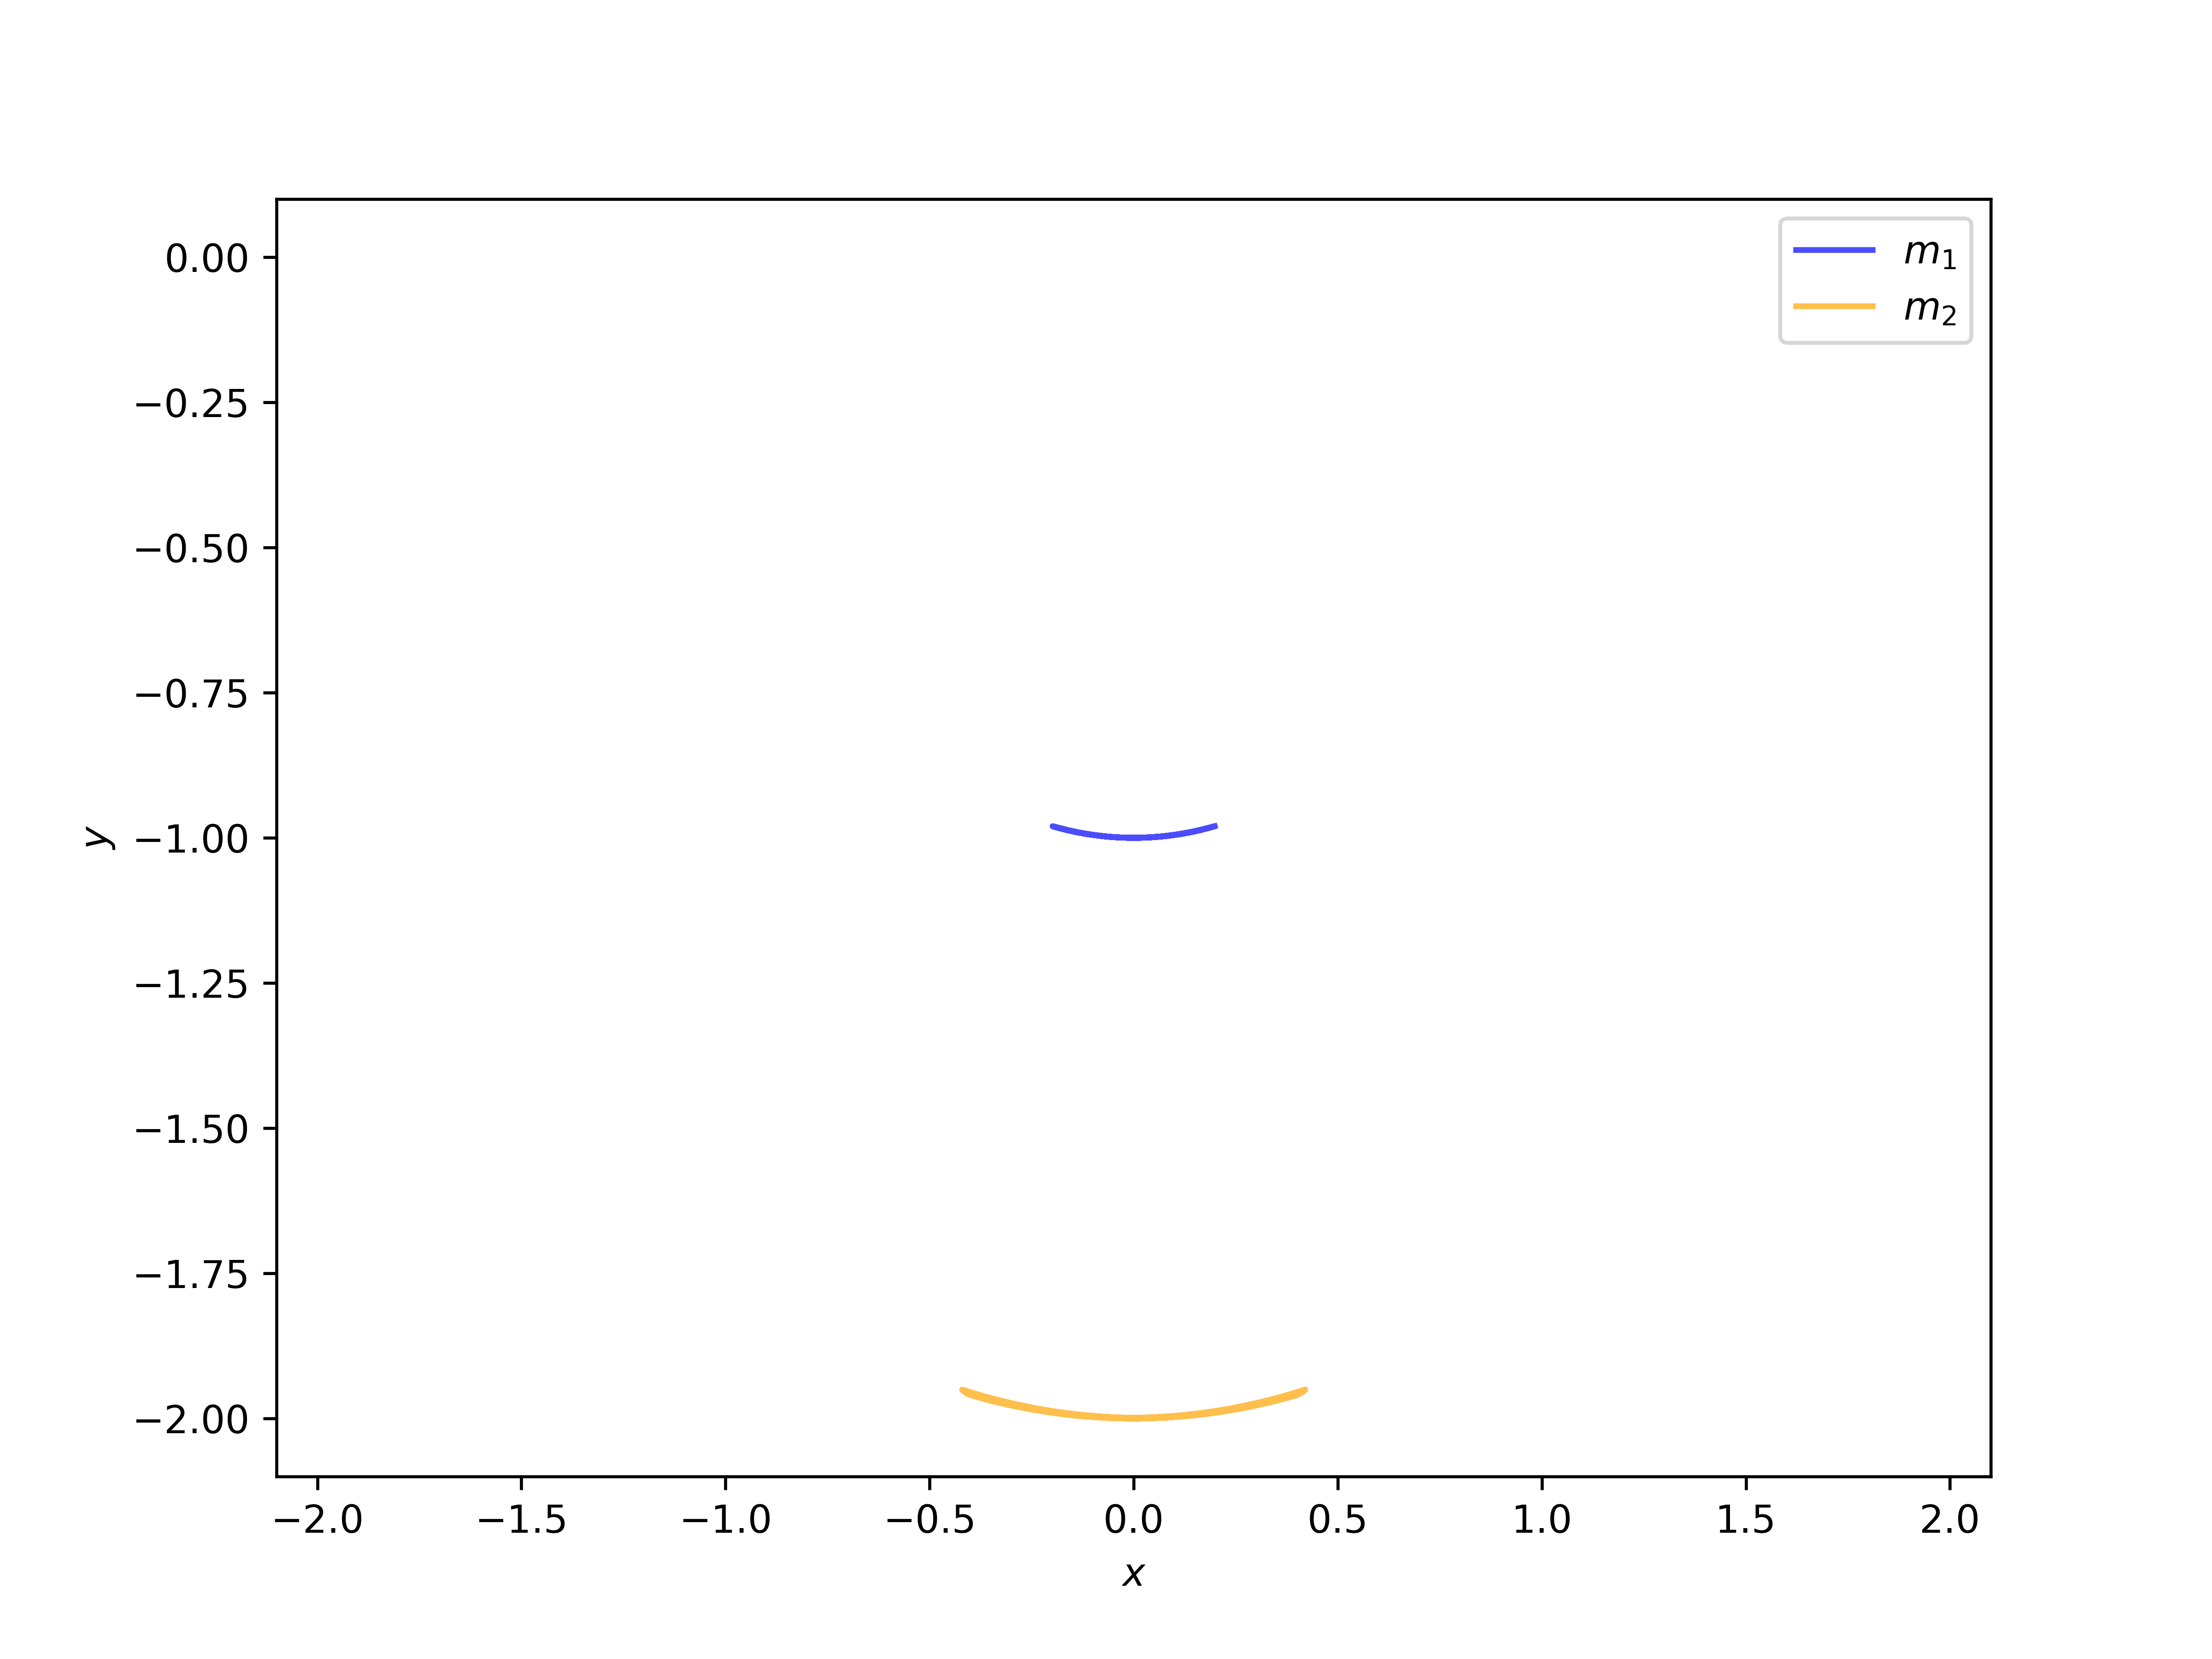
\includegraphics[width=5.5cm]{img/double_pendulum_path_nc.png} }}%
    \qquad
    \subfloat[Double pendulum angle over time.]{{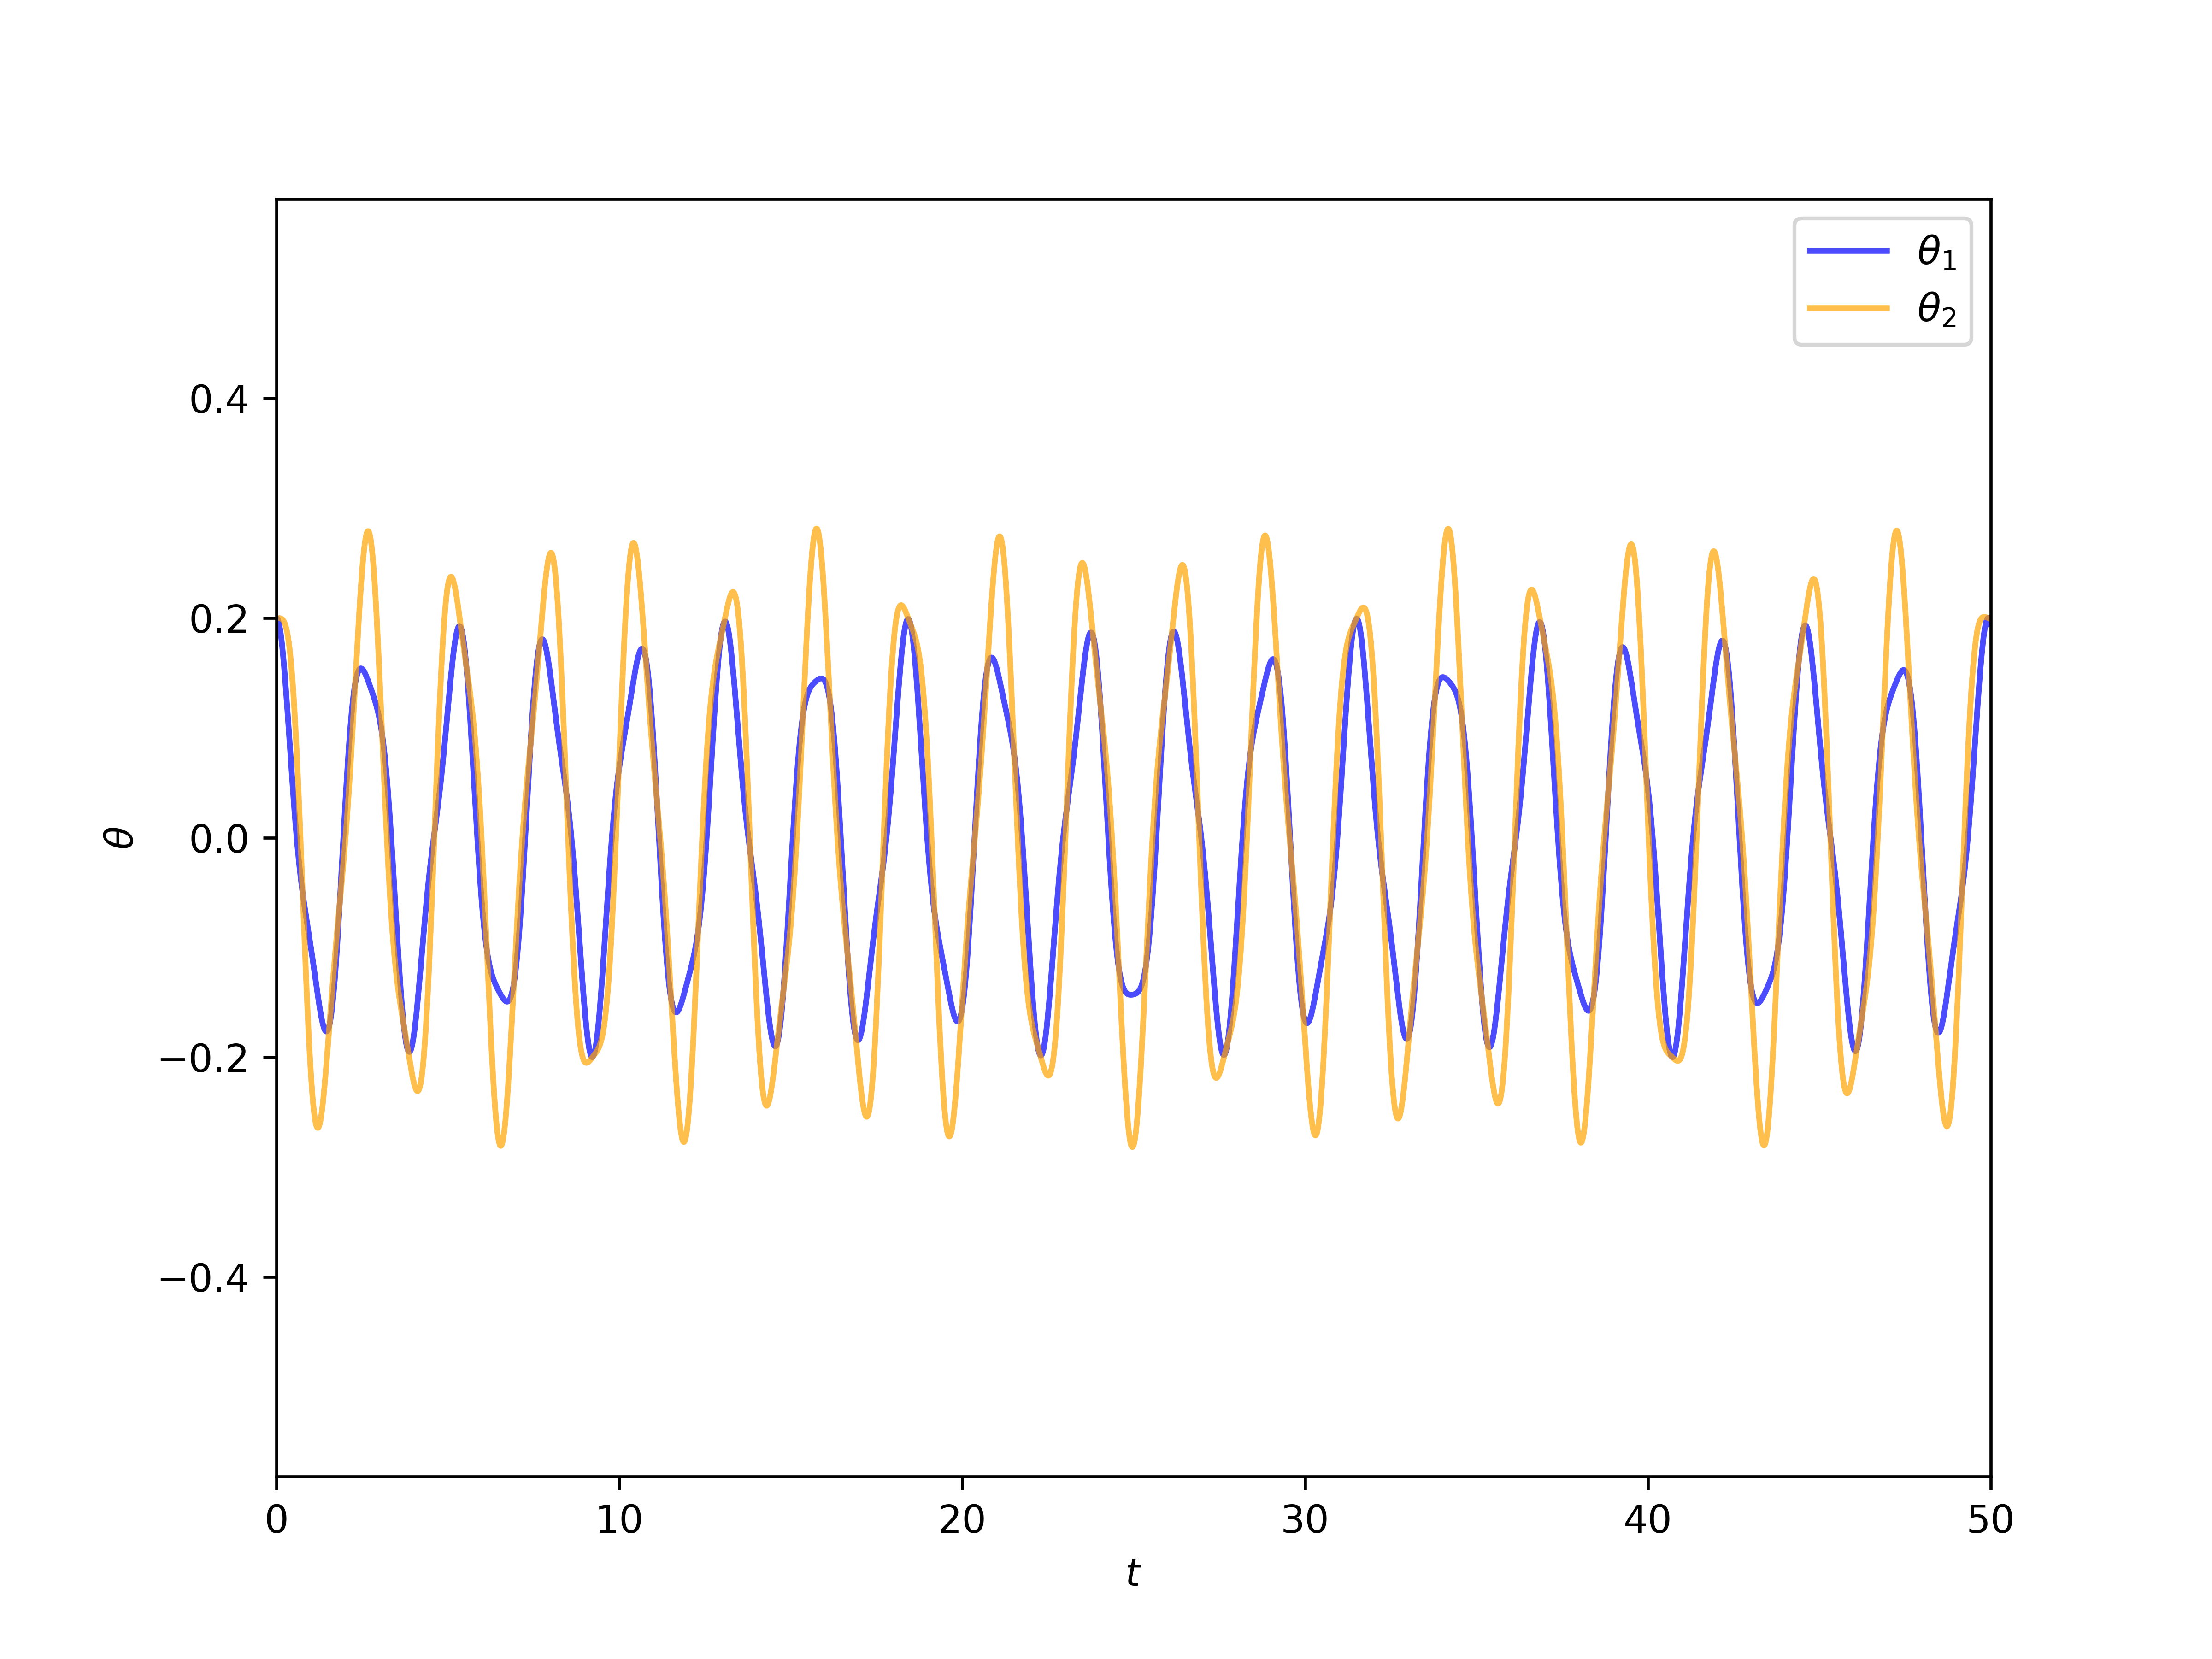
\includegraphics[width=5.5cm]{img/double_pendulum_angle_nc.png} }}%
    \caption{The double pendulum with small initial angles}%
    \label{fig:example}%
\end{figure}

Here in this Figure, this is the first simulation output of a double pendulum. Based on the path lines, it looks very similar to the simple pendulum. The pendulum bobs do not deviate away from the circle the bob was restricted to in the simple pendulum case. For this case gravity overpowers the initial conditions and does not allow for the second, yellow pendulum bob to move out of order. \\

In Figure (b) above, the sinusoidal pattern is seen again. However, in this case it is not nearly as perfect. Since the different masses now have an effect on each other, perfect harmonic motion is near impossible. This system is still not chaotic despite the discrepancy in the motion.


\begin{figure}%
    \centering
    \subfloat[Simple pendulum bob path.]{{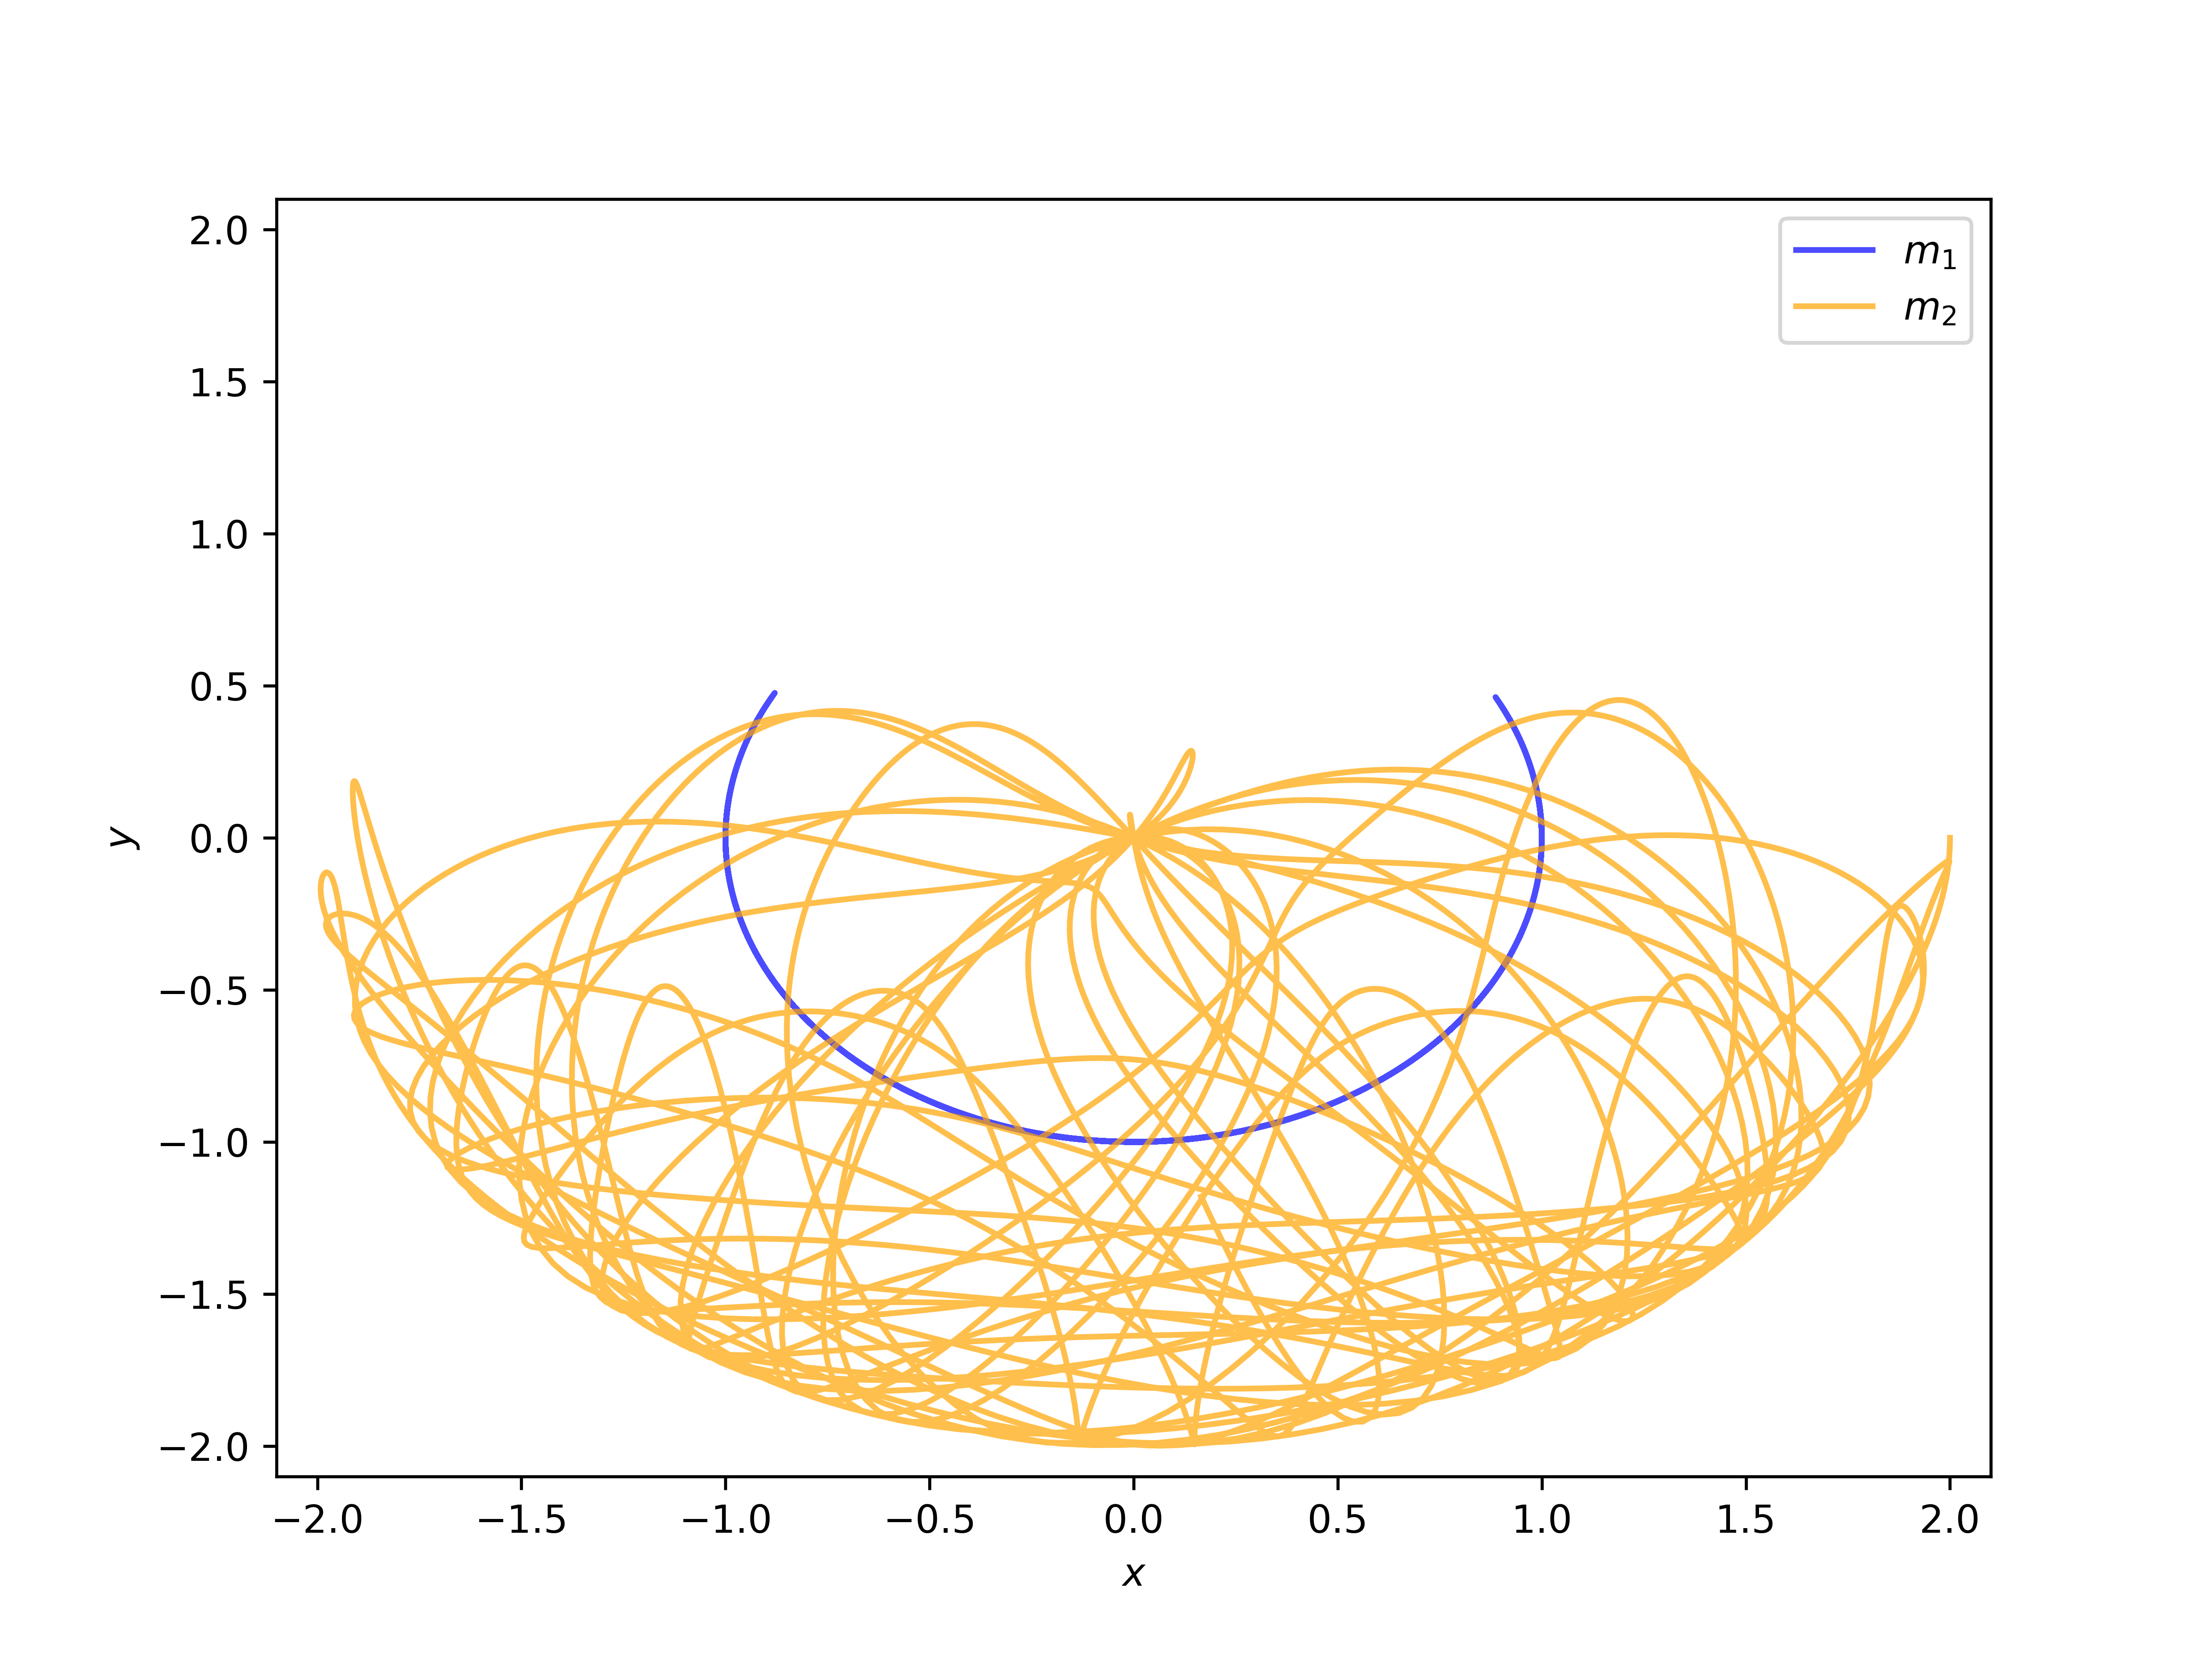
\includegraphics[width=5.5cm]{img/double_pendulum_path_pi2.png} }}%
    \qquad
    \subfloat[Simple pendulum angle over time.]{{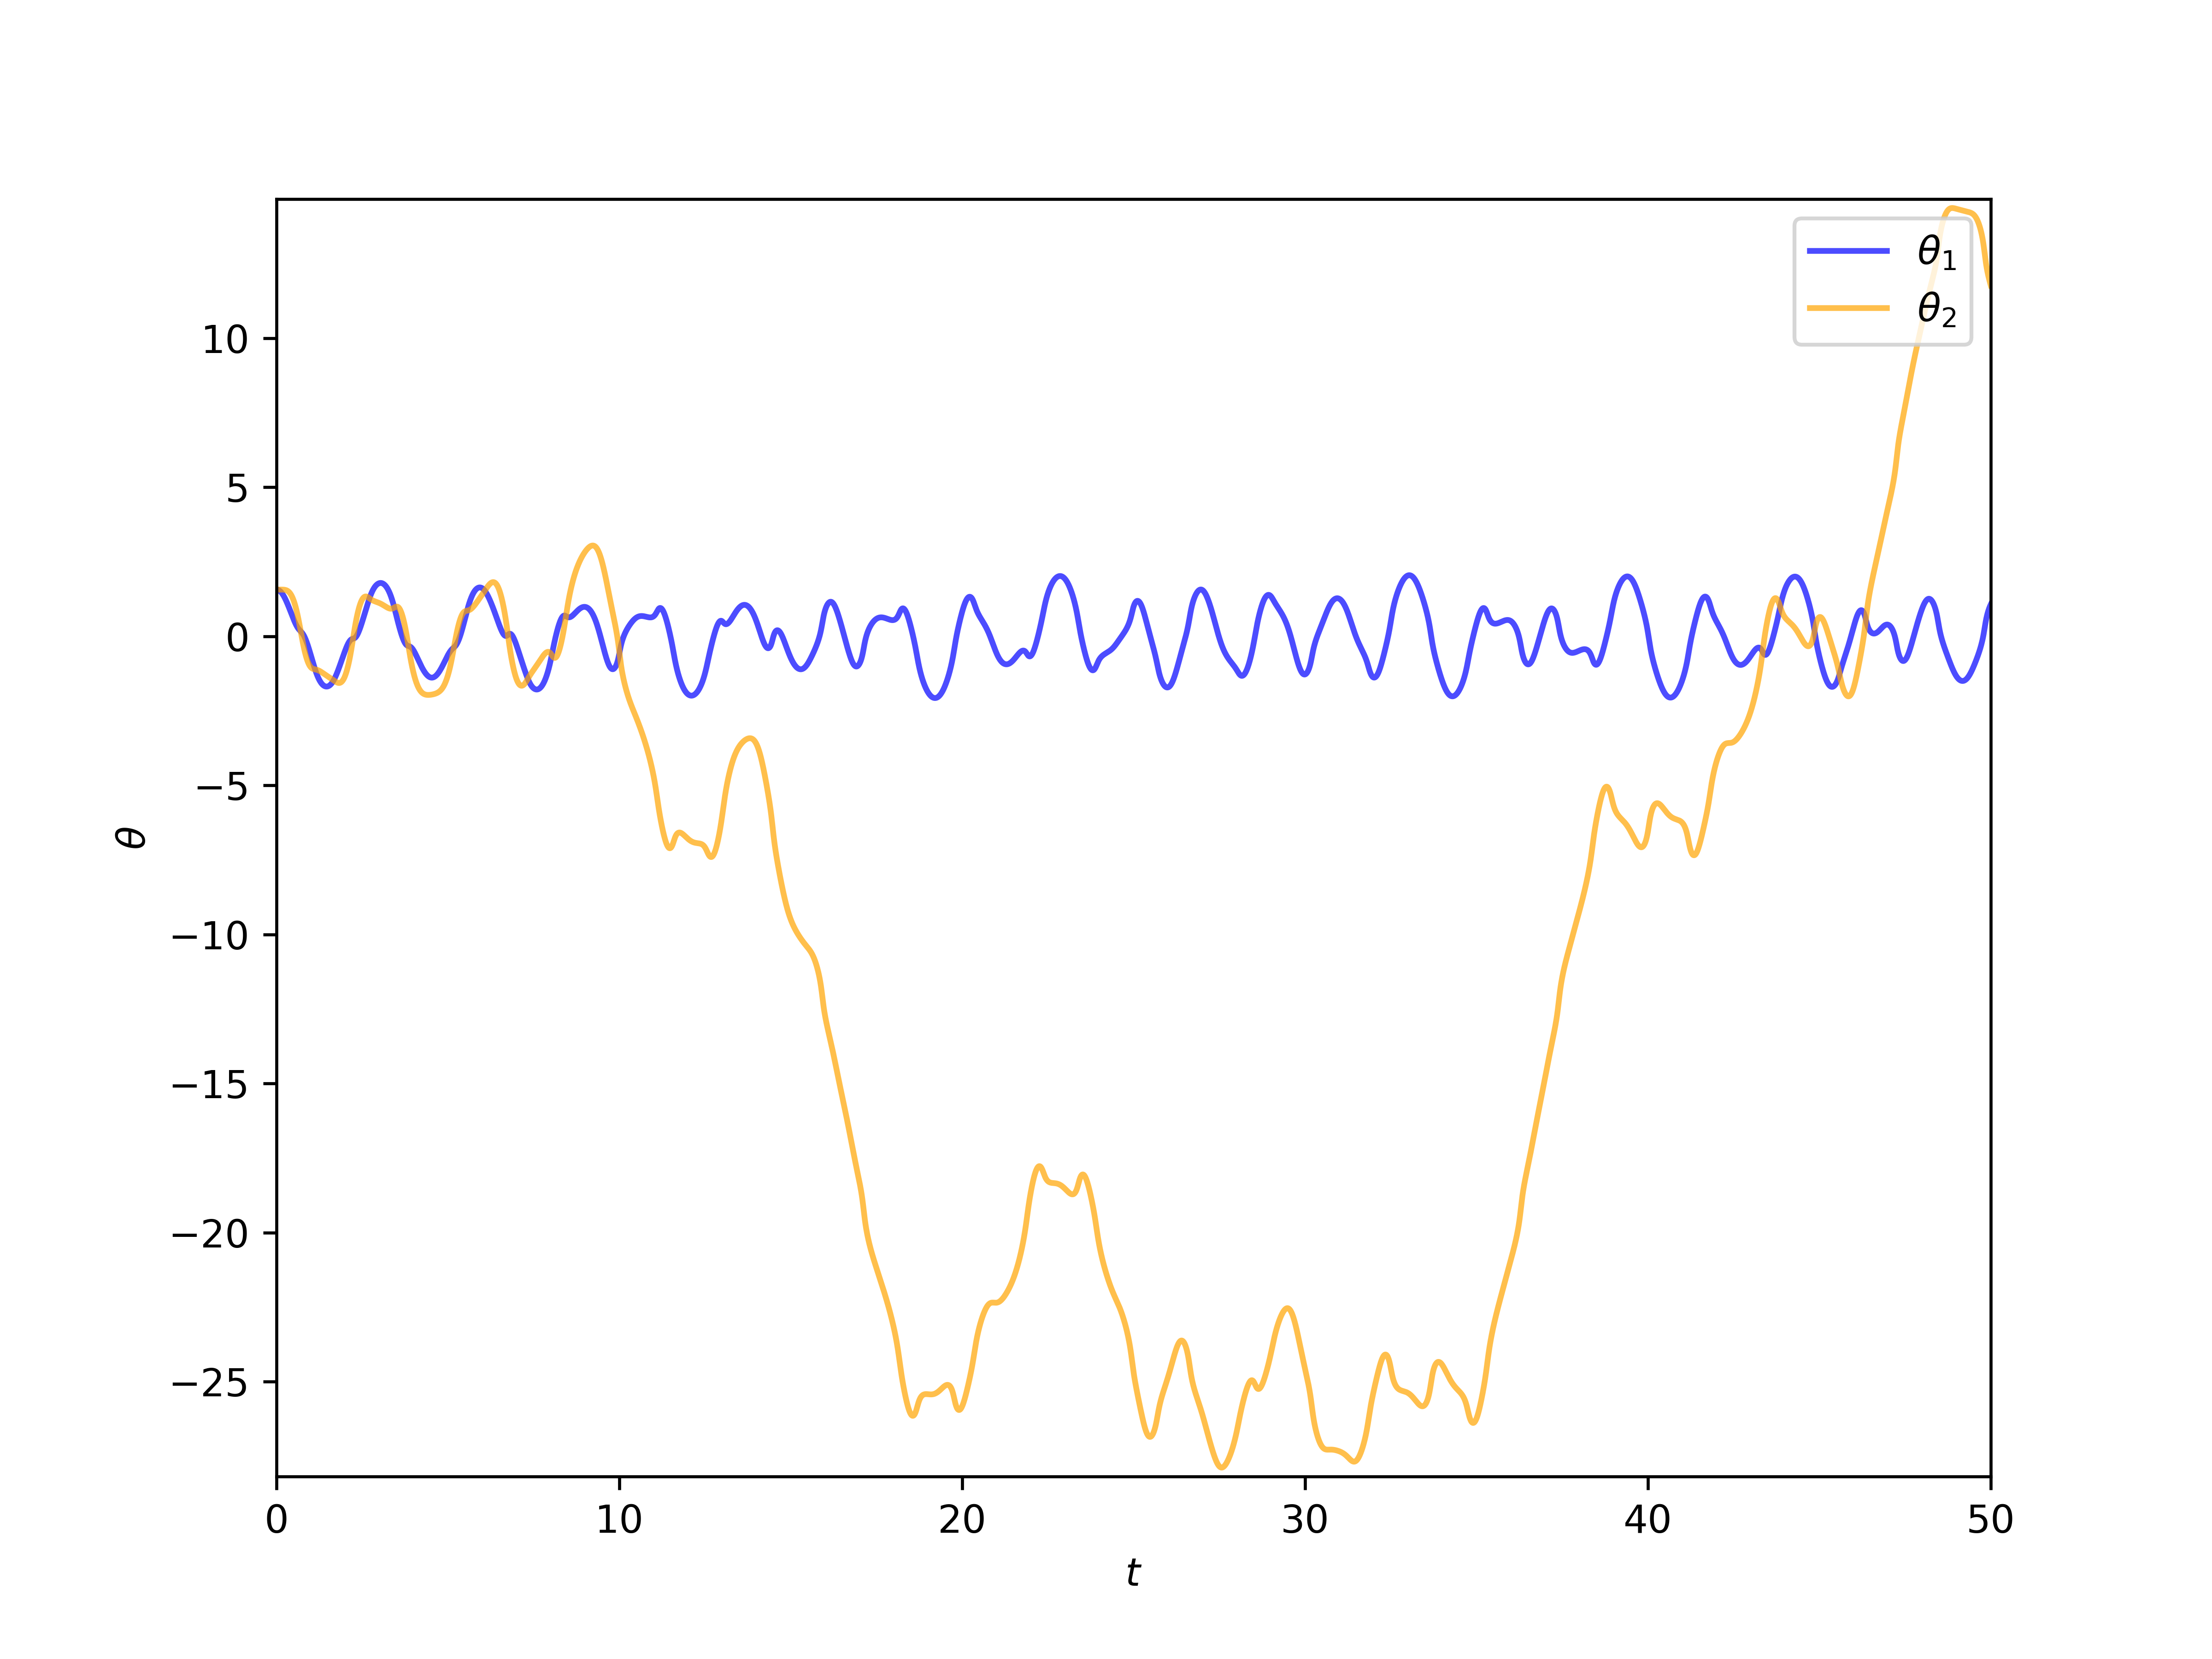
\includegraphics[width=5.5cm]{img/double_pendulum_angle_pi2.png} }}%
    \caption{The double pendulum model with large initial angles}%
    \label{fig:example}%
\end{figure}

Increasing the initial angle of the pendulum begins the chaos.


\begin{figure}%
    \centering
    \subfloat[Simple pendulum bob path.]{{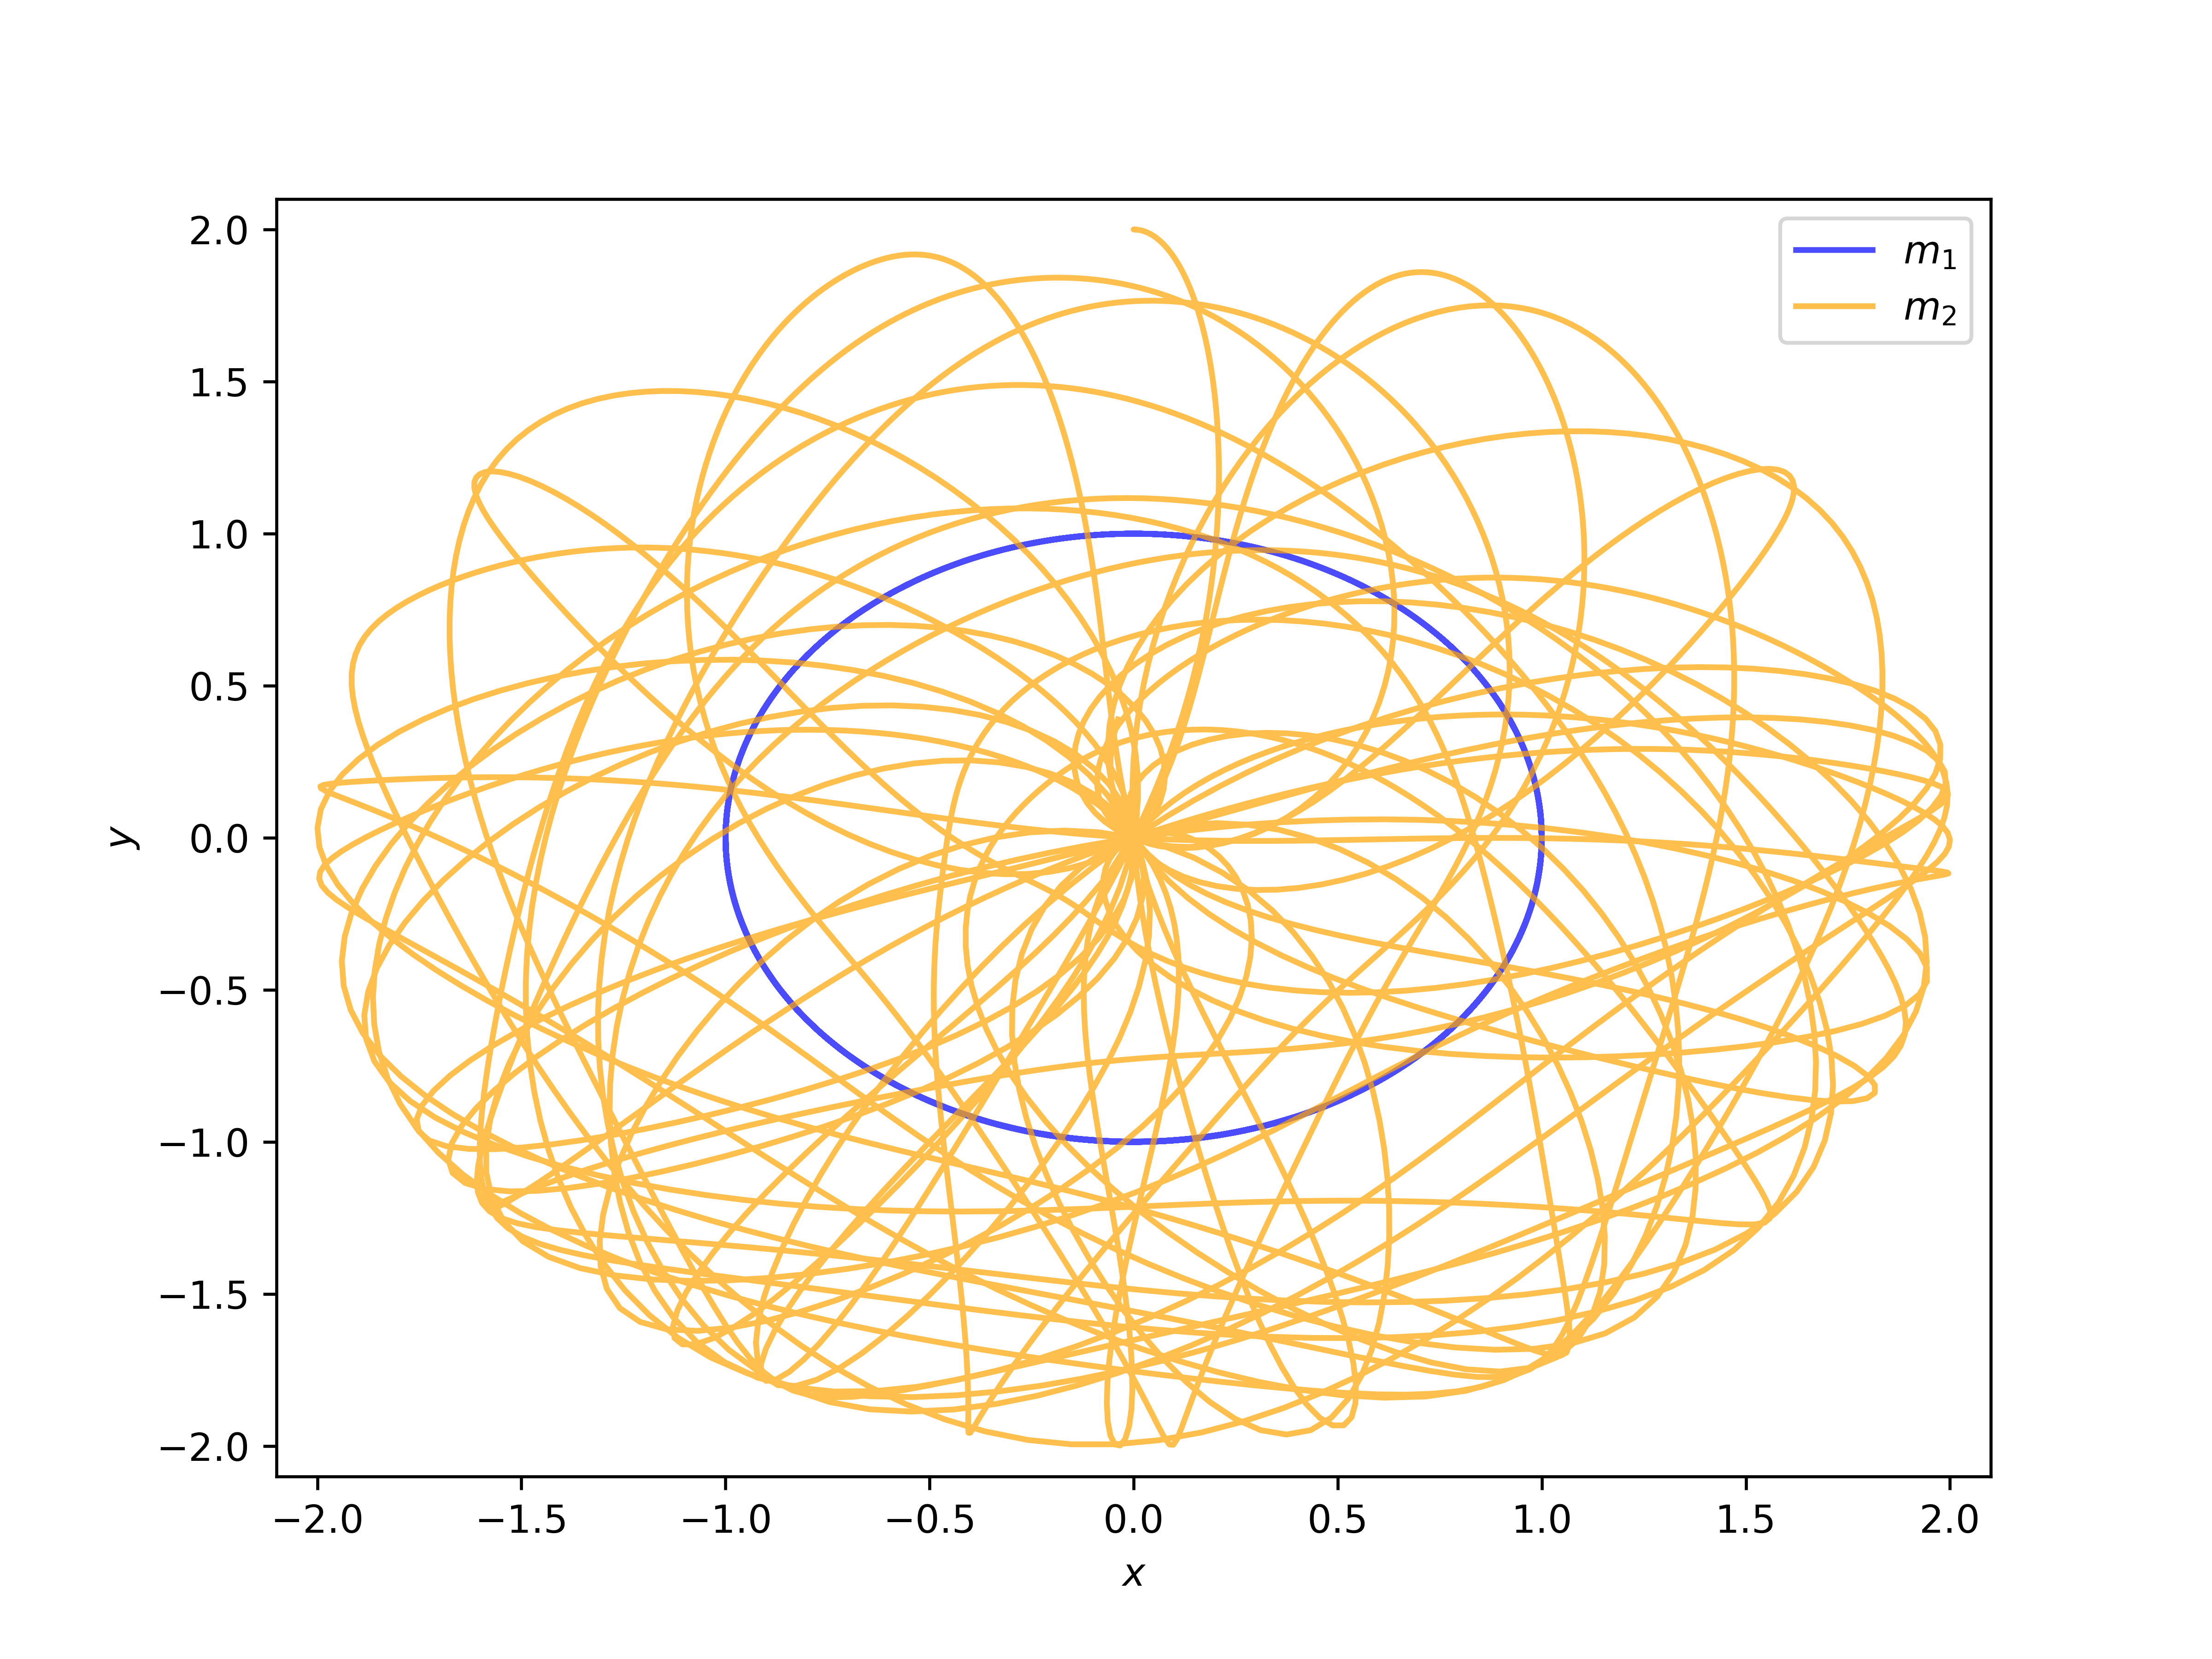
\includegraphics[width=5.5cm]{img/double_pendulum_path_neg_pi.png} }}%
    \qquad
    \subfloat[Simple pendulum angle over time.]{{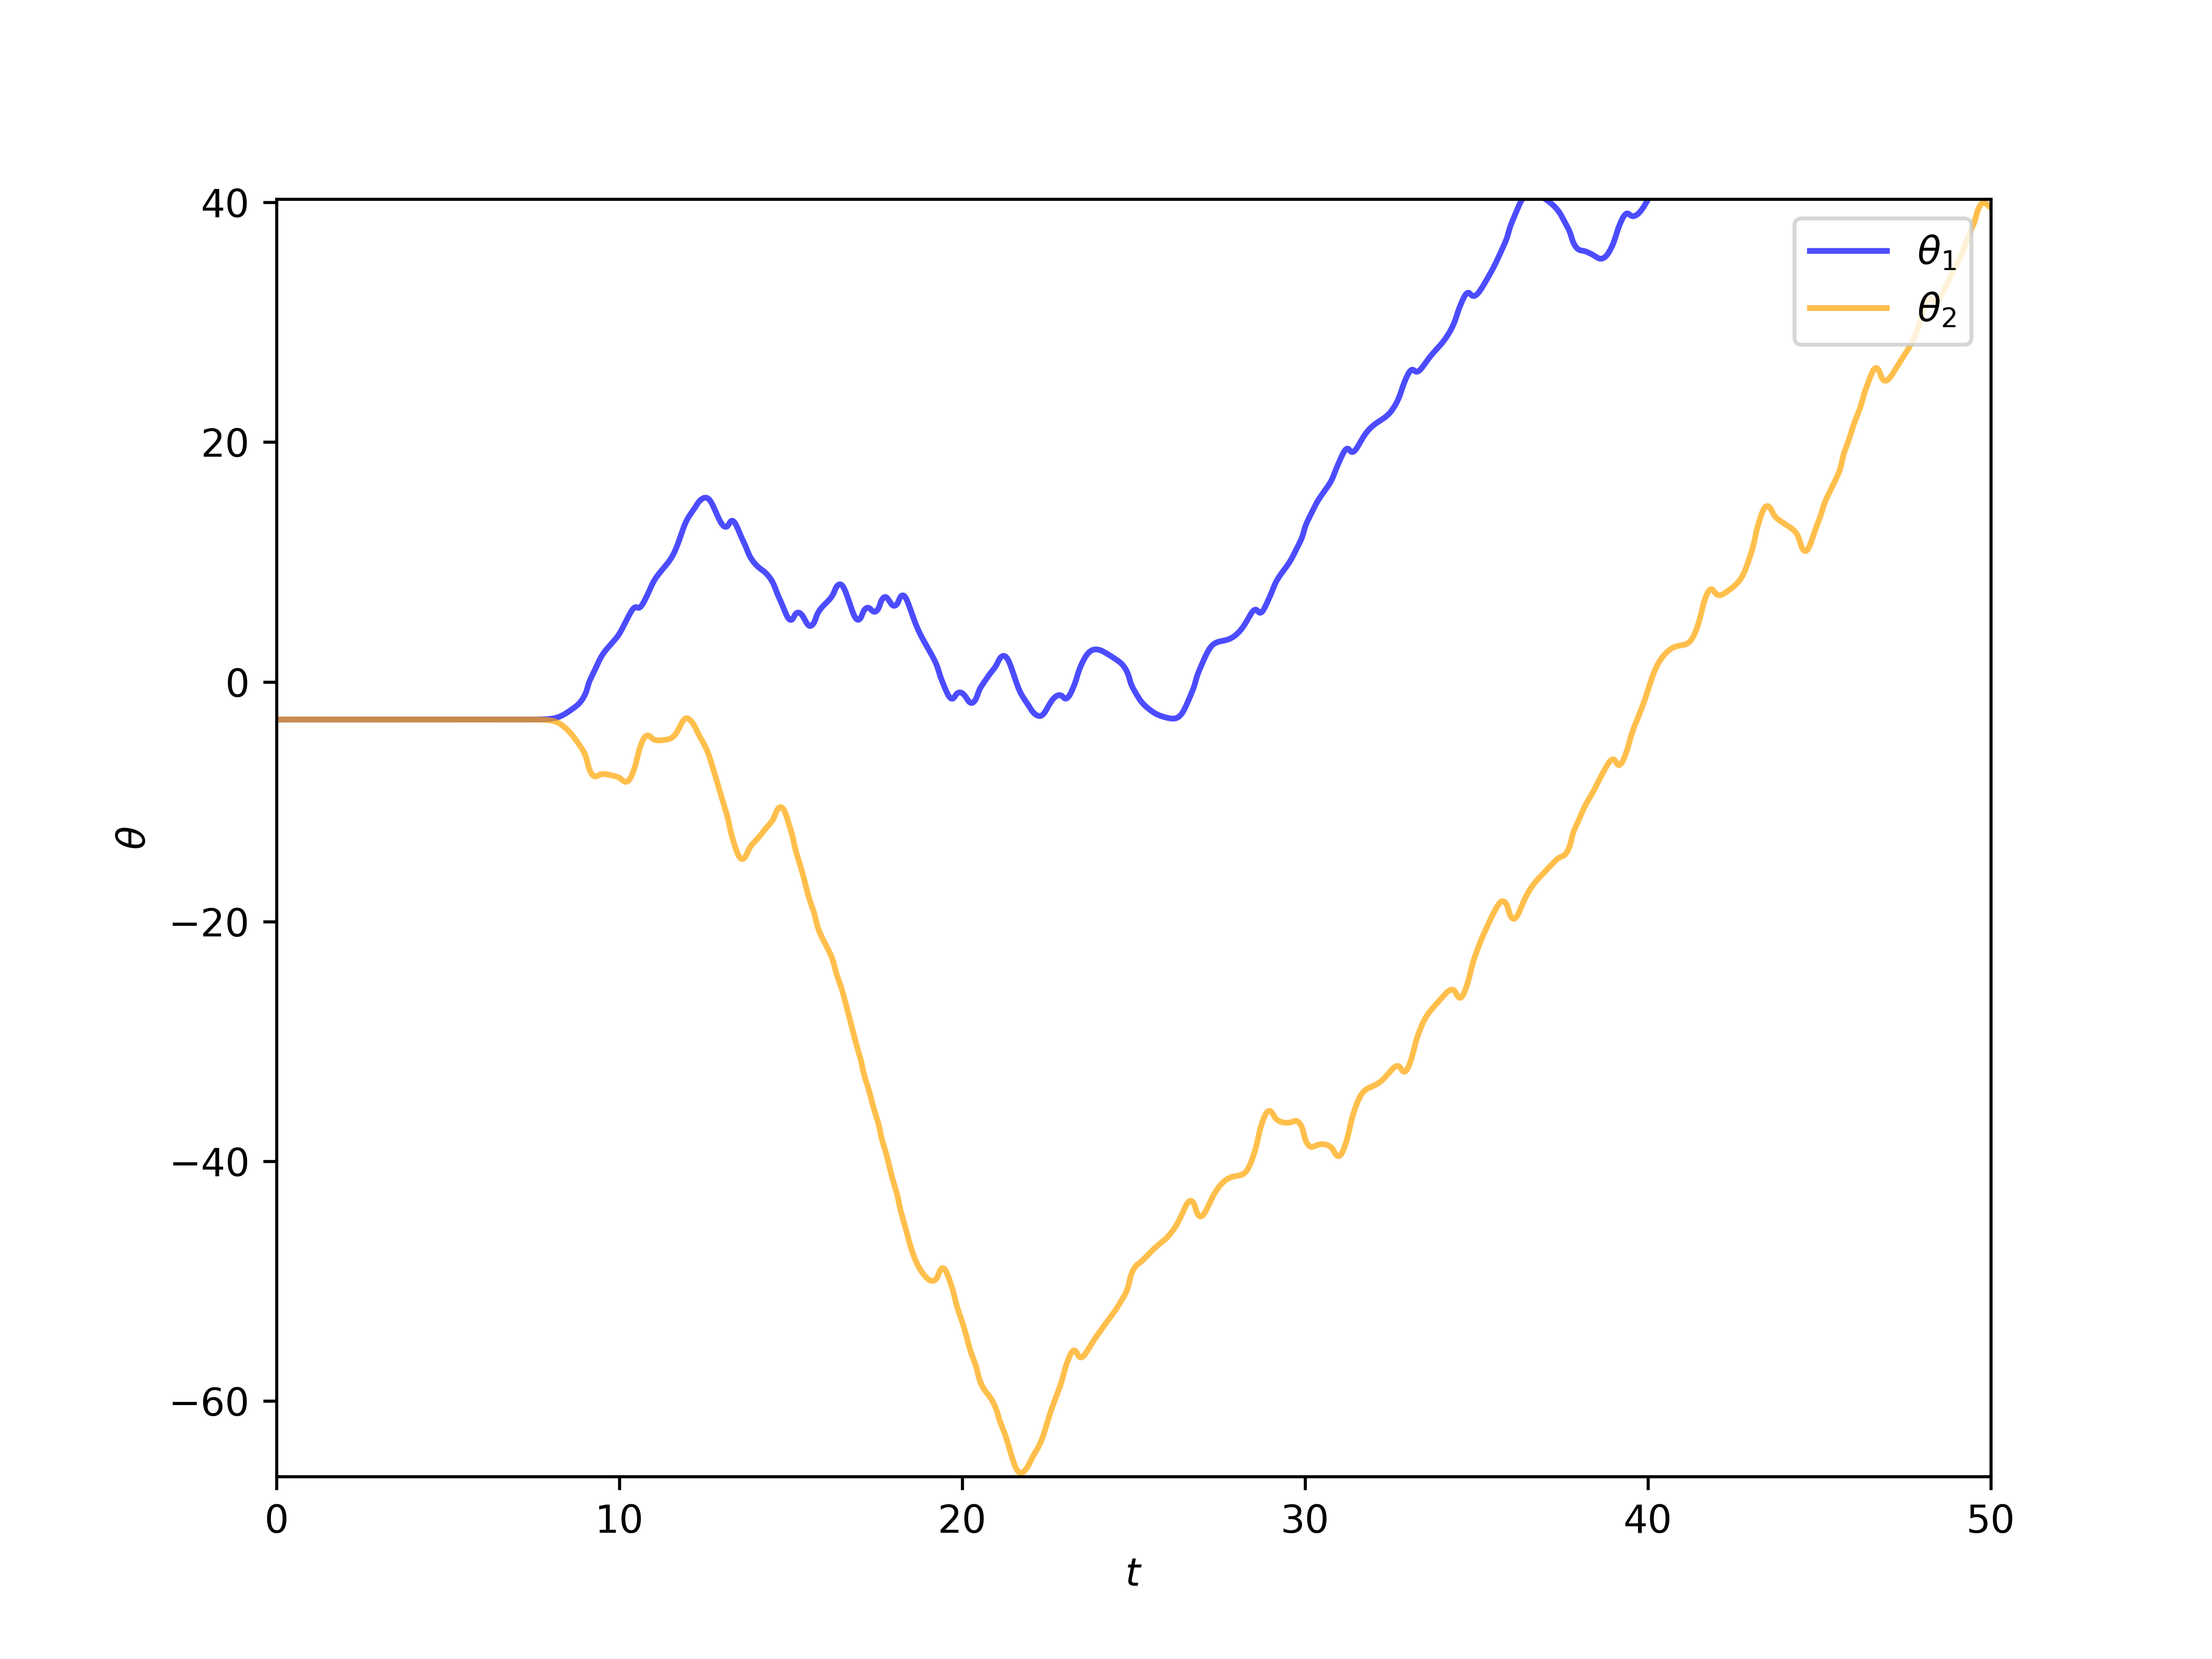
\includegraphics[width=5.5cm]{img/double_pendulum_angle_neg_pi.png} }}%
    \caption{The double pendulum in an unstable state.}%
    \label{fig:example}%
\end{figure}

This last figure shows the first 10 seconds of the theta vs time plot in an unstable state. The model starts the pendulum mass in a perfect 90 degree start. Over the course of the first 10 seconds the double pendulum is stuck in this position. After the 10 second the numerical model finds stability and the model continues in its stable form and the chaos of the pendulum is formed. 

\subsubsection{Chaos Theory Arises.}

The figures in the previous section show visually just how chaotic a double pendulum can be. A good question to ask is how chaotic is a double pendulum and what is chaos theory at its core? A common misconception in chaos theory is that a system is never predictable. Meaning that no matter what level of understanding the system there is no predicting what the system may do. Furthermore, if the system were to run with the same parameters the outcome of the system will be entirely different than in the previous run. Nonetheless, thinking of chaos theory in this way is absolutely wrong. \\

Chaos theory can be deterministic with the double pendulum system. If there is a set of establish initial conditions, then the system can be integrated forward in time with the utmost precision. Chaos theory, at its core for this system, has exceedingly different results based on different initial conditions over time. \\

The modelling theory of chaos with the double pendulum is alluring but not always practical. The experimental side of this theory quickly meets limitations. There becomes an excessive amount of error introduced when trying to run this experiment physically. Error builds with time as the experiment runs and we lose the infinite precision we had with a computer. Regardless, it becomes apparent in the computational model and the physical experiment on how minuscule changes in the system have profound outcomes. \\

\subsubsection{The Model.}

\begin{figure}[h]
    \centering
    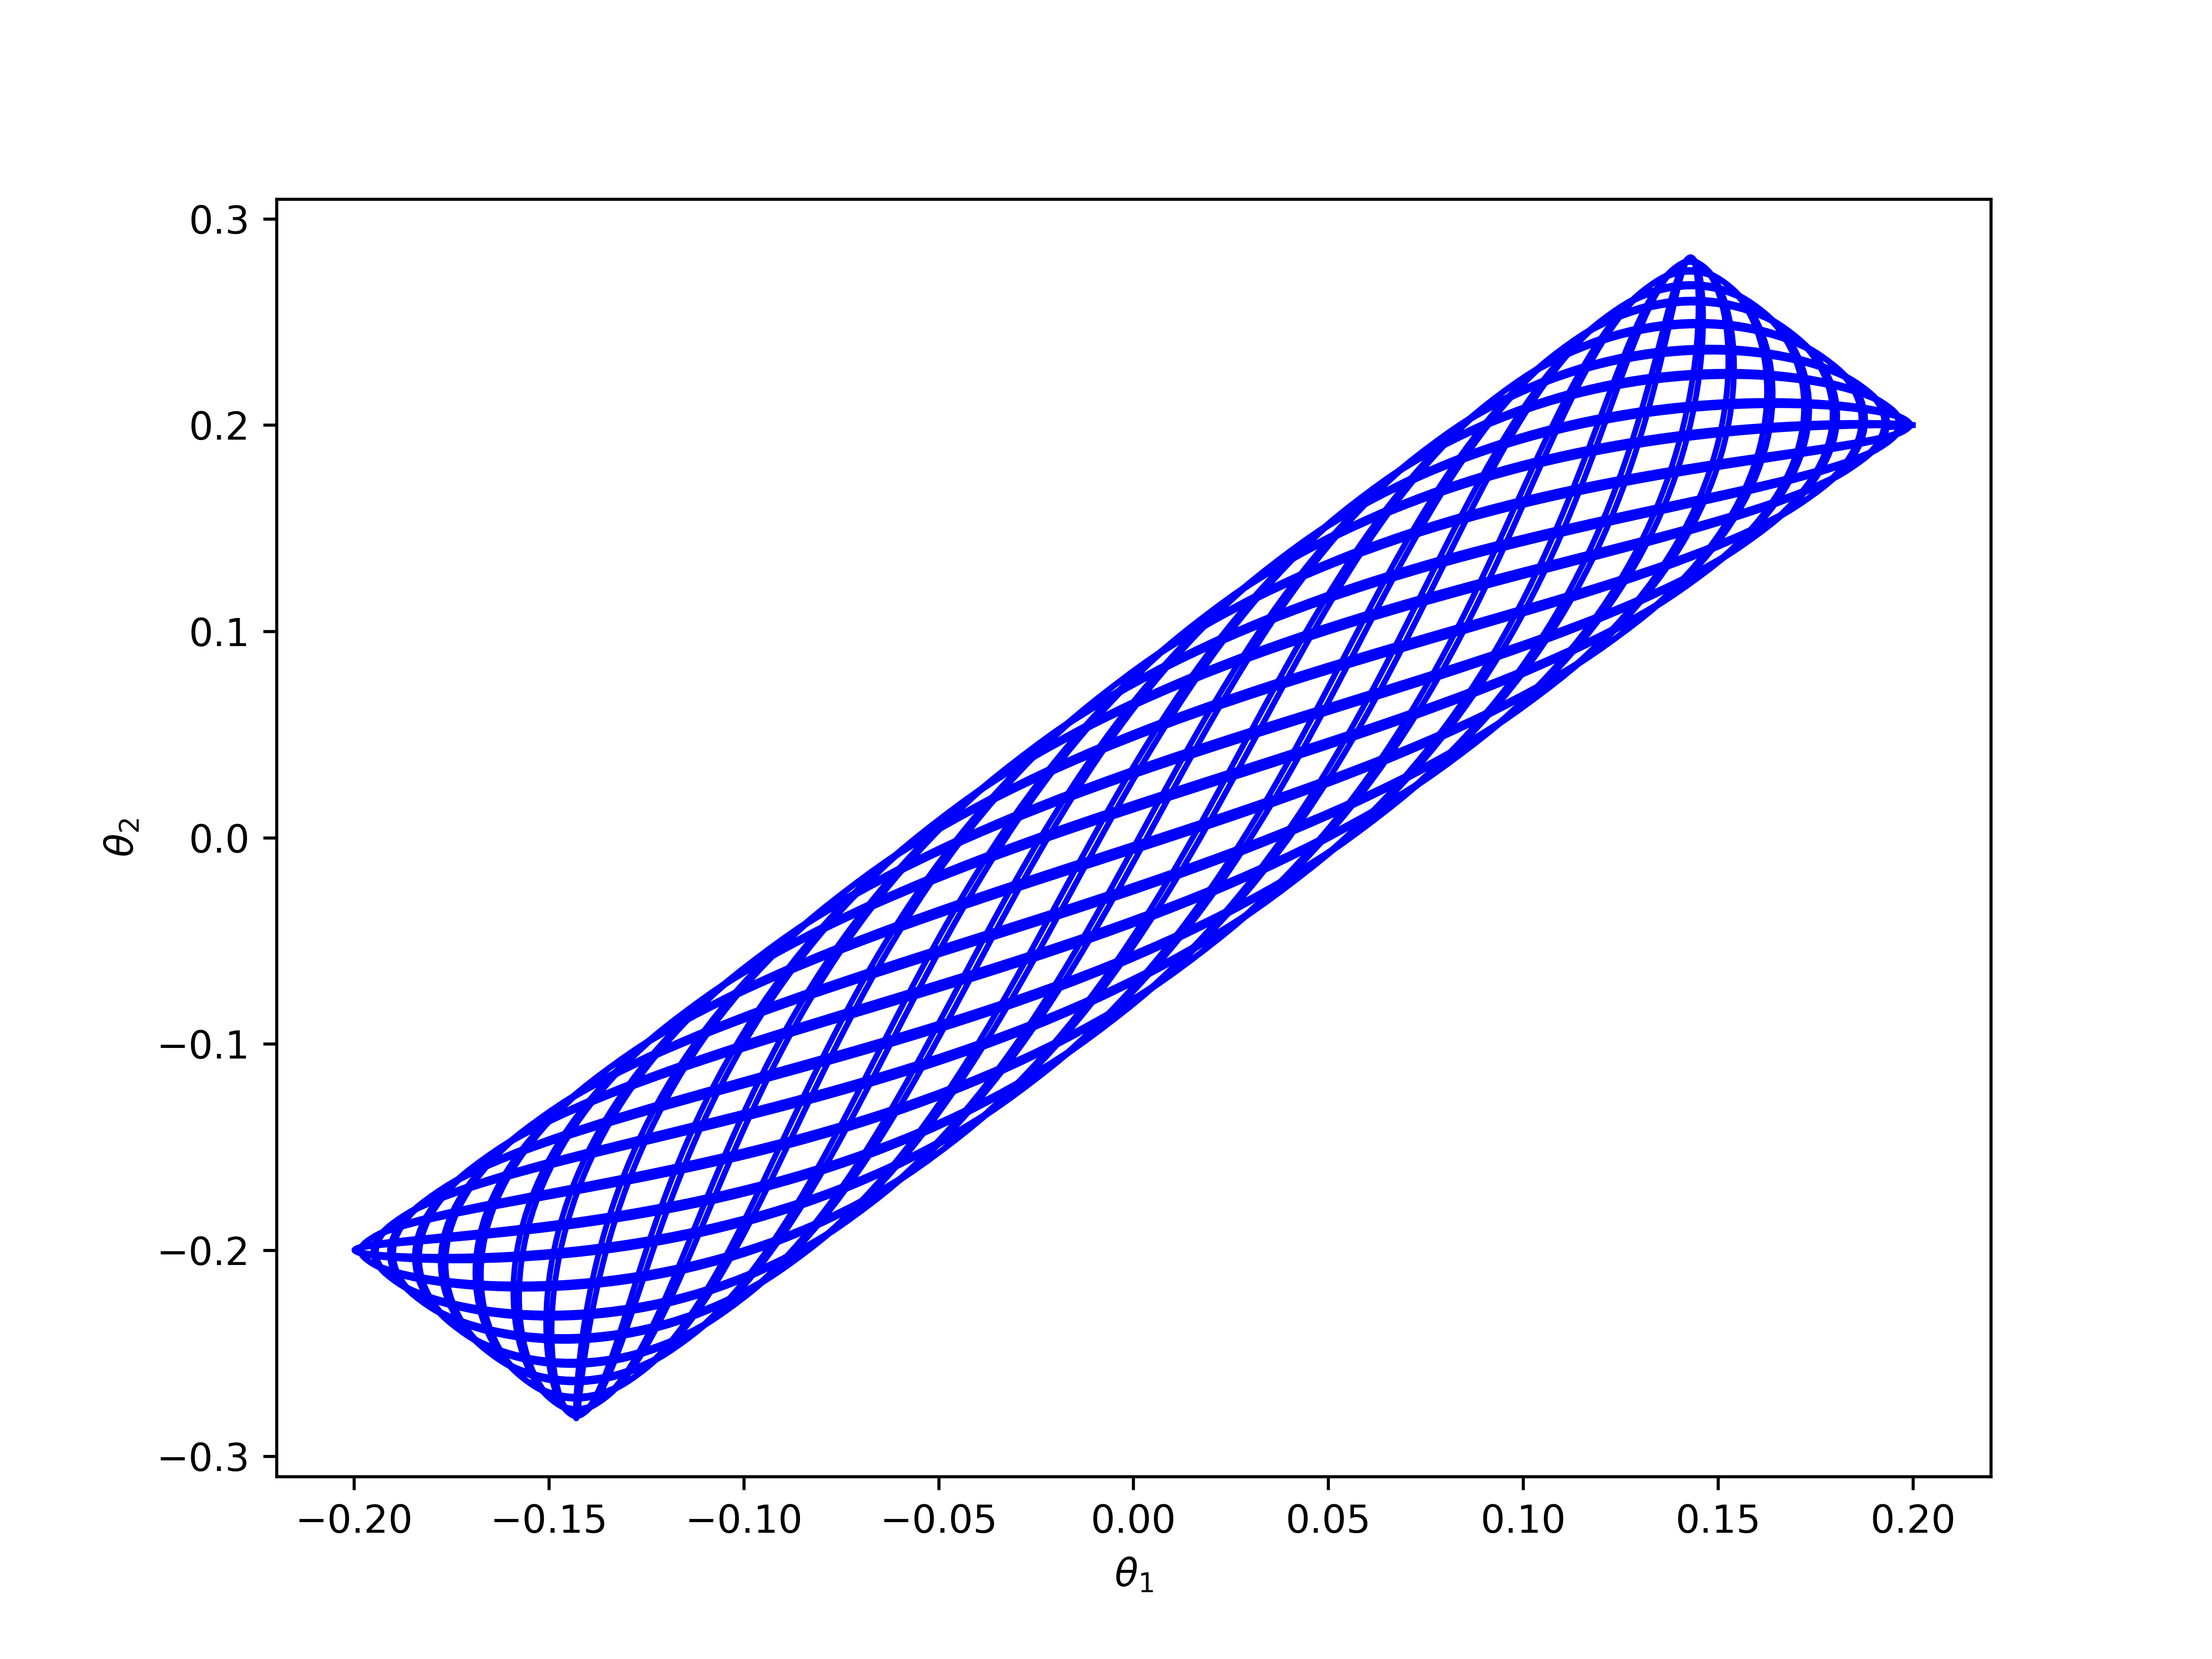
\includegraphics[width=0.75\textwidth]{img/simple_pendulum_thetas_non_chaos.png}
    \caption{A $\theta_1$ vs $\theta_2$ plot}
    \label{fig:theta_vs_theta}
\end{figure}
 
 The Figure above shows a plot that plots $\theta_1$ vs $\theta_2$. For this run in the model, the conditions were set to have near perfect harmonic motion and to rule out chaos. Therefore, this run had close to perfect oscillation for both angles. The figure above is a representation of a pattern that in return shows how non-chaotic the conditions were. In a sense this is very close to how the simple pendulum moved. 



\begin{figure}[!htb]
\minipage{0.32\textwidth}
  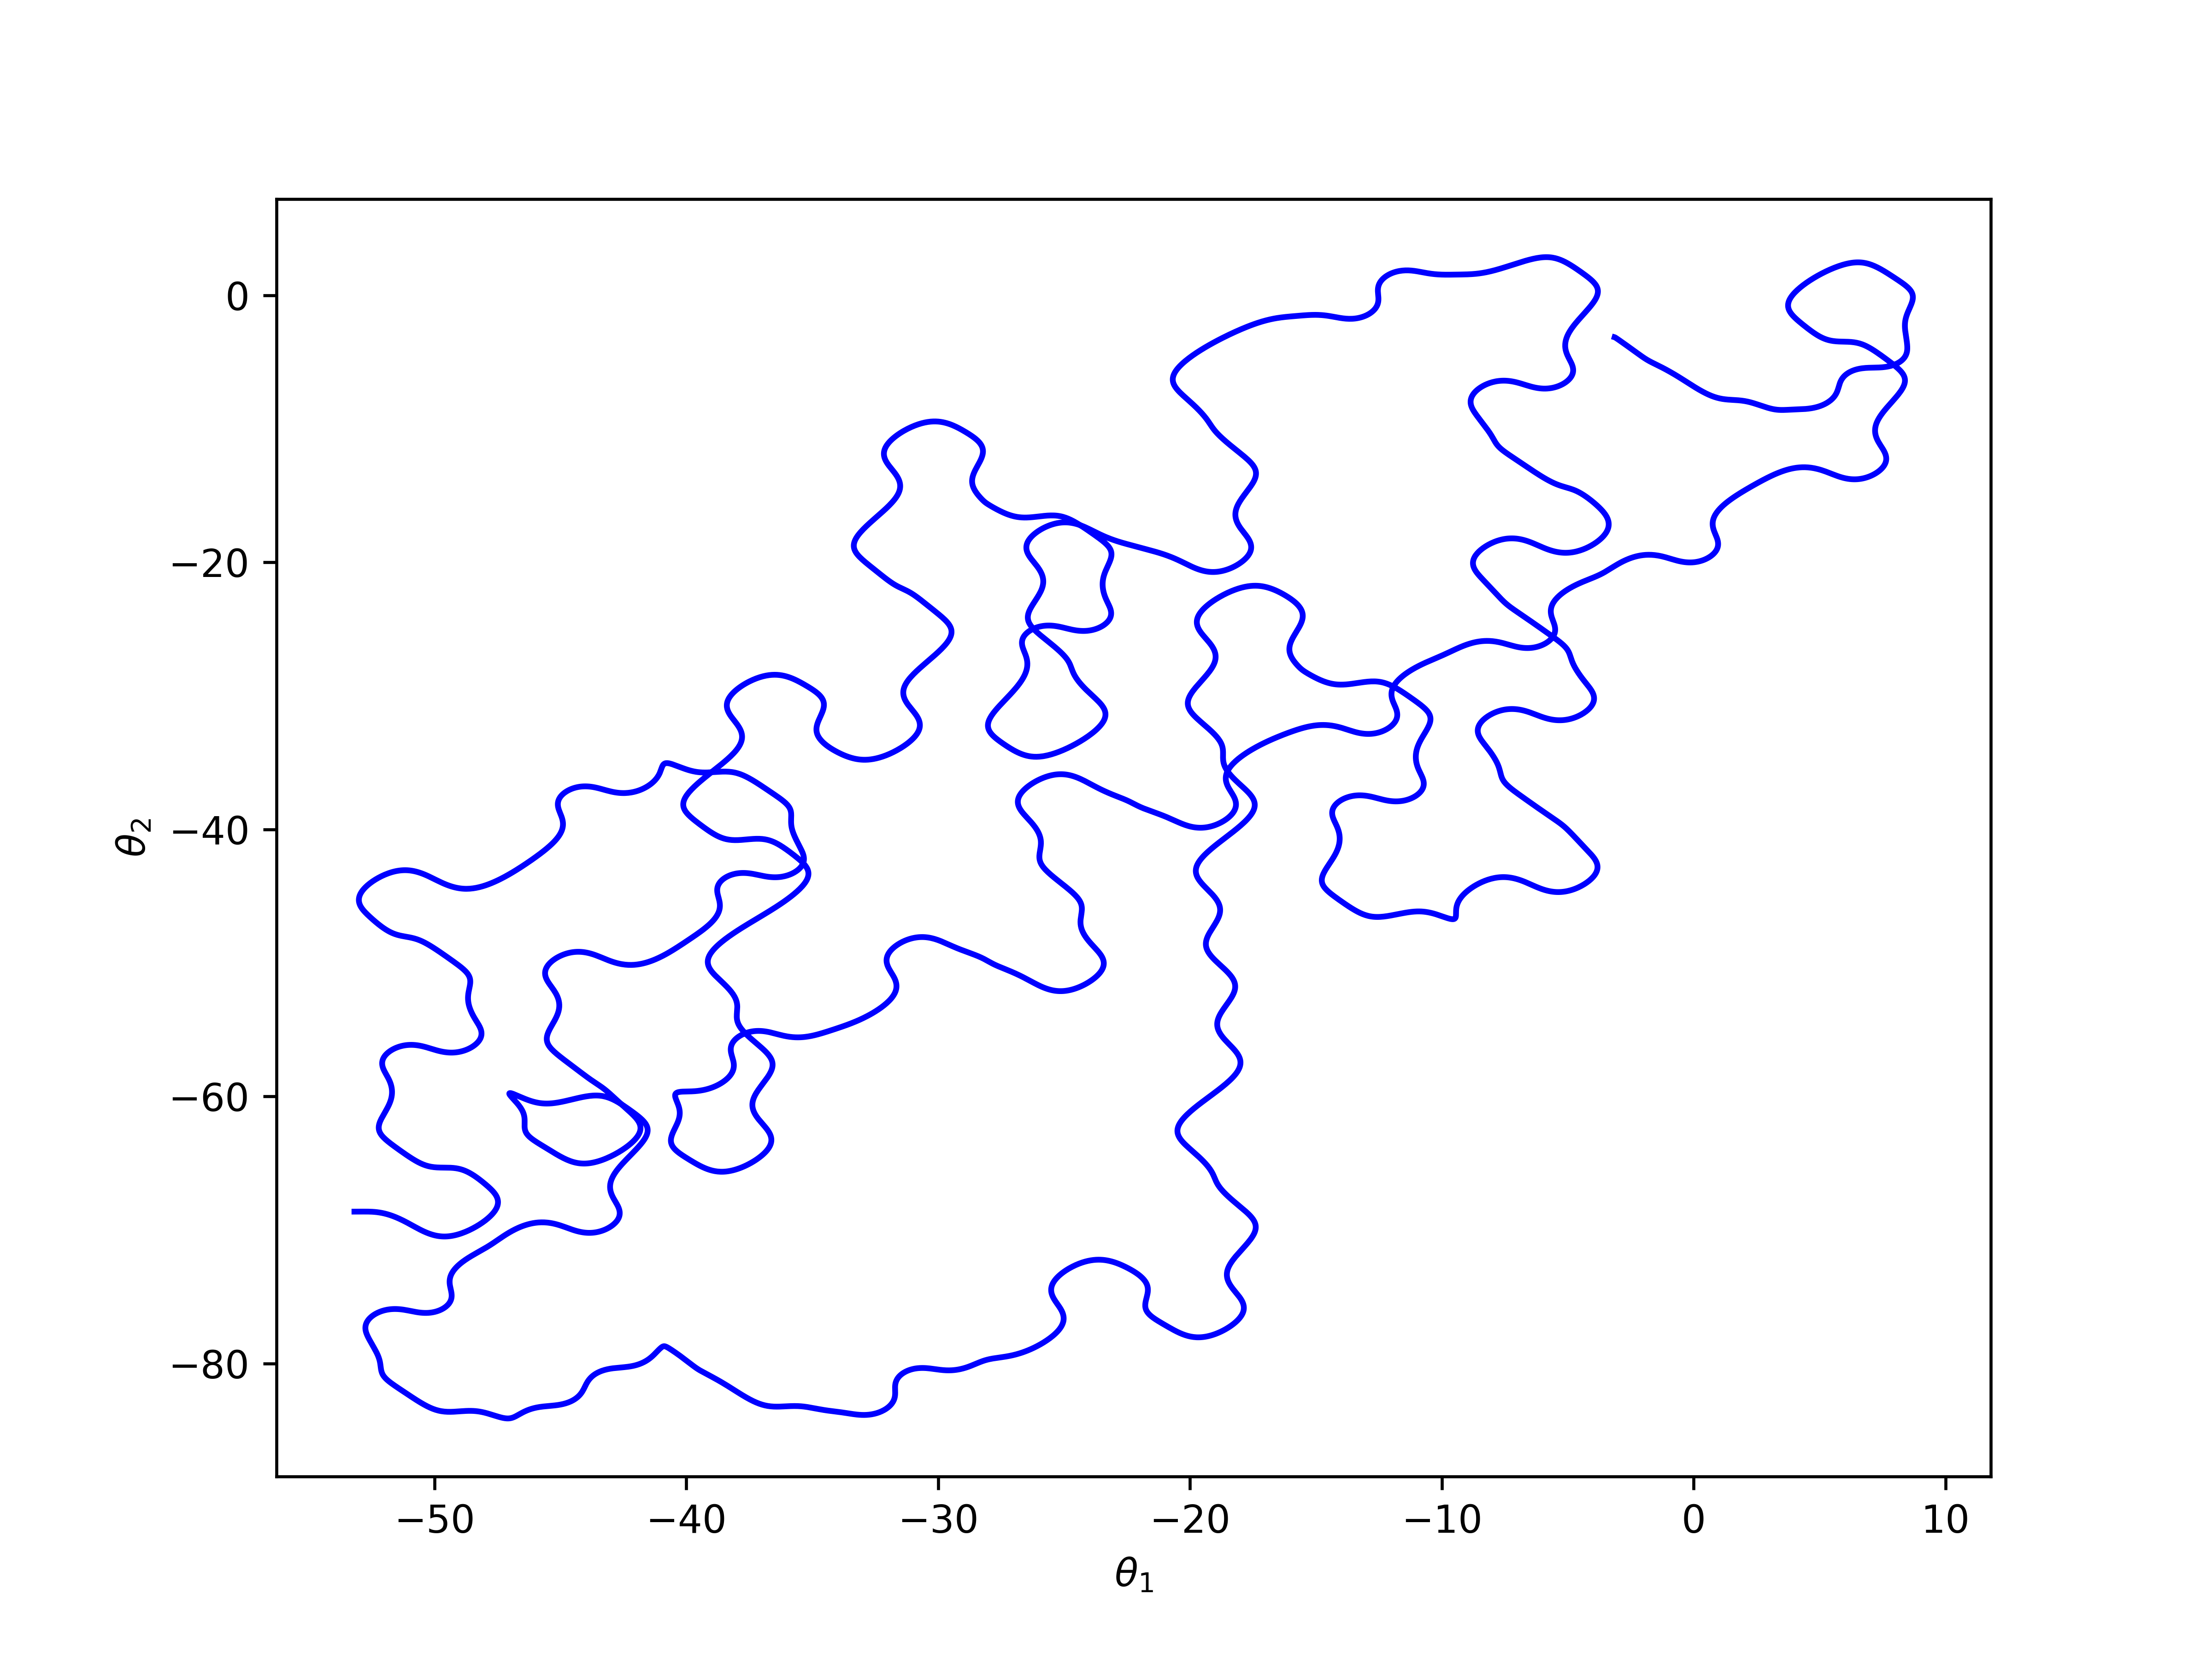
\includegraphics[width=\linewidth]{img/theta_theta_1.png}
  \caption{Pendulum 1 $\theta_1$ vs $\theta_2$.}\label{fig:theta_vs_theta_1}
\endminipage\hfill
\minipage{0.32\textwidth}
  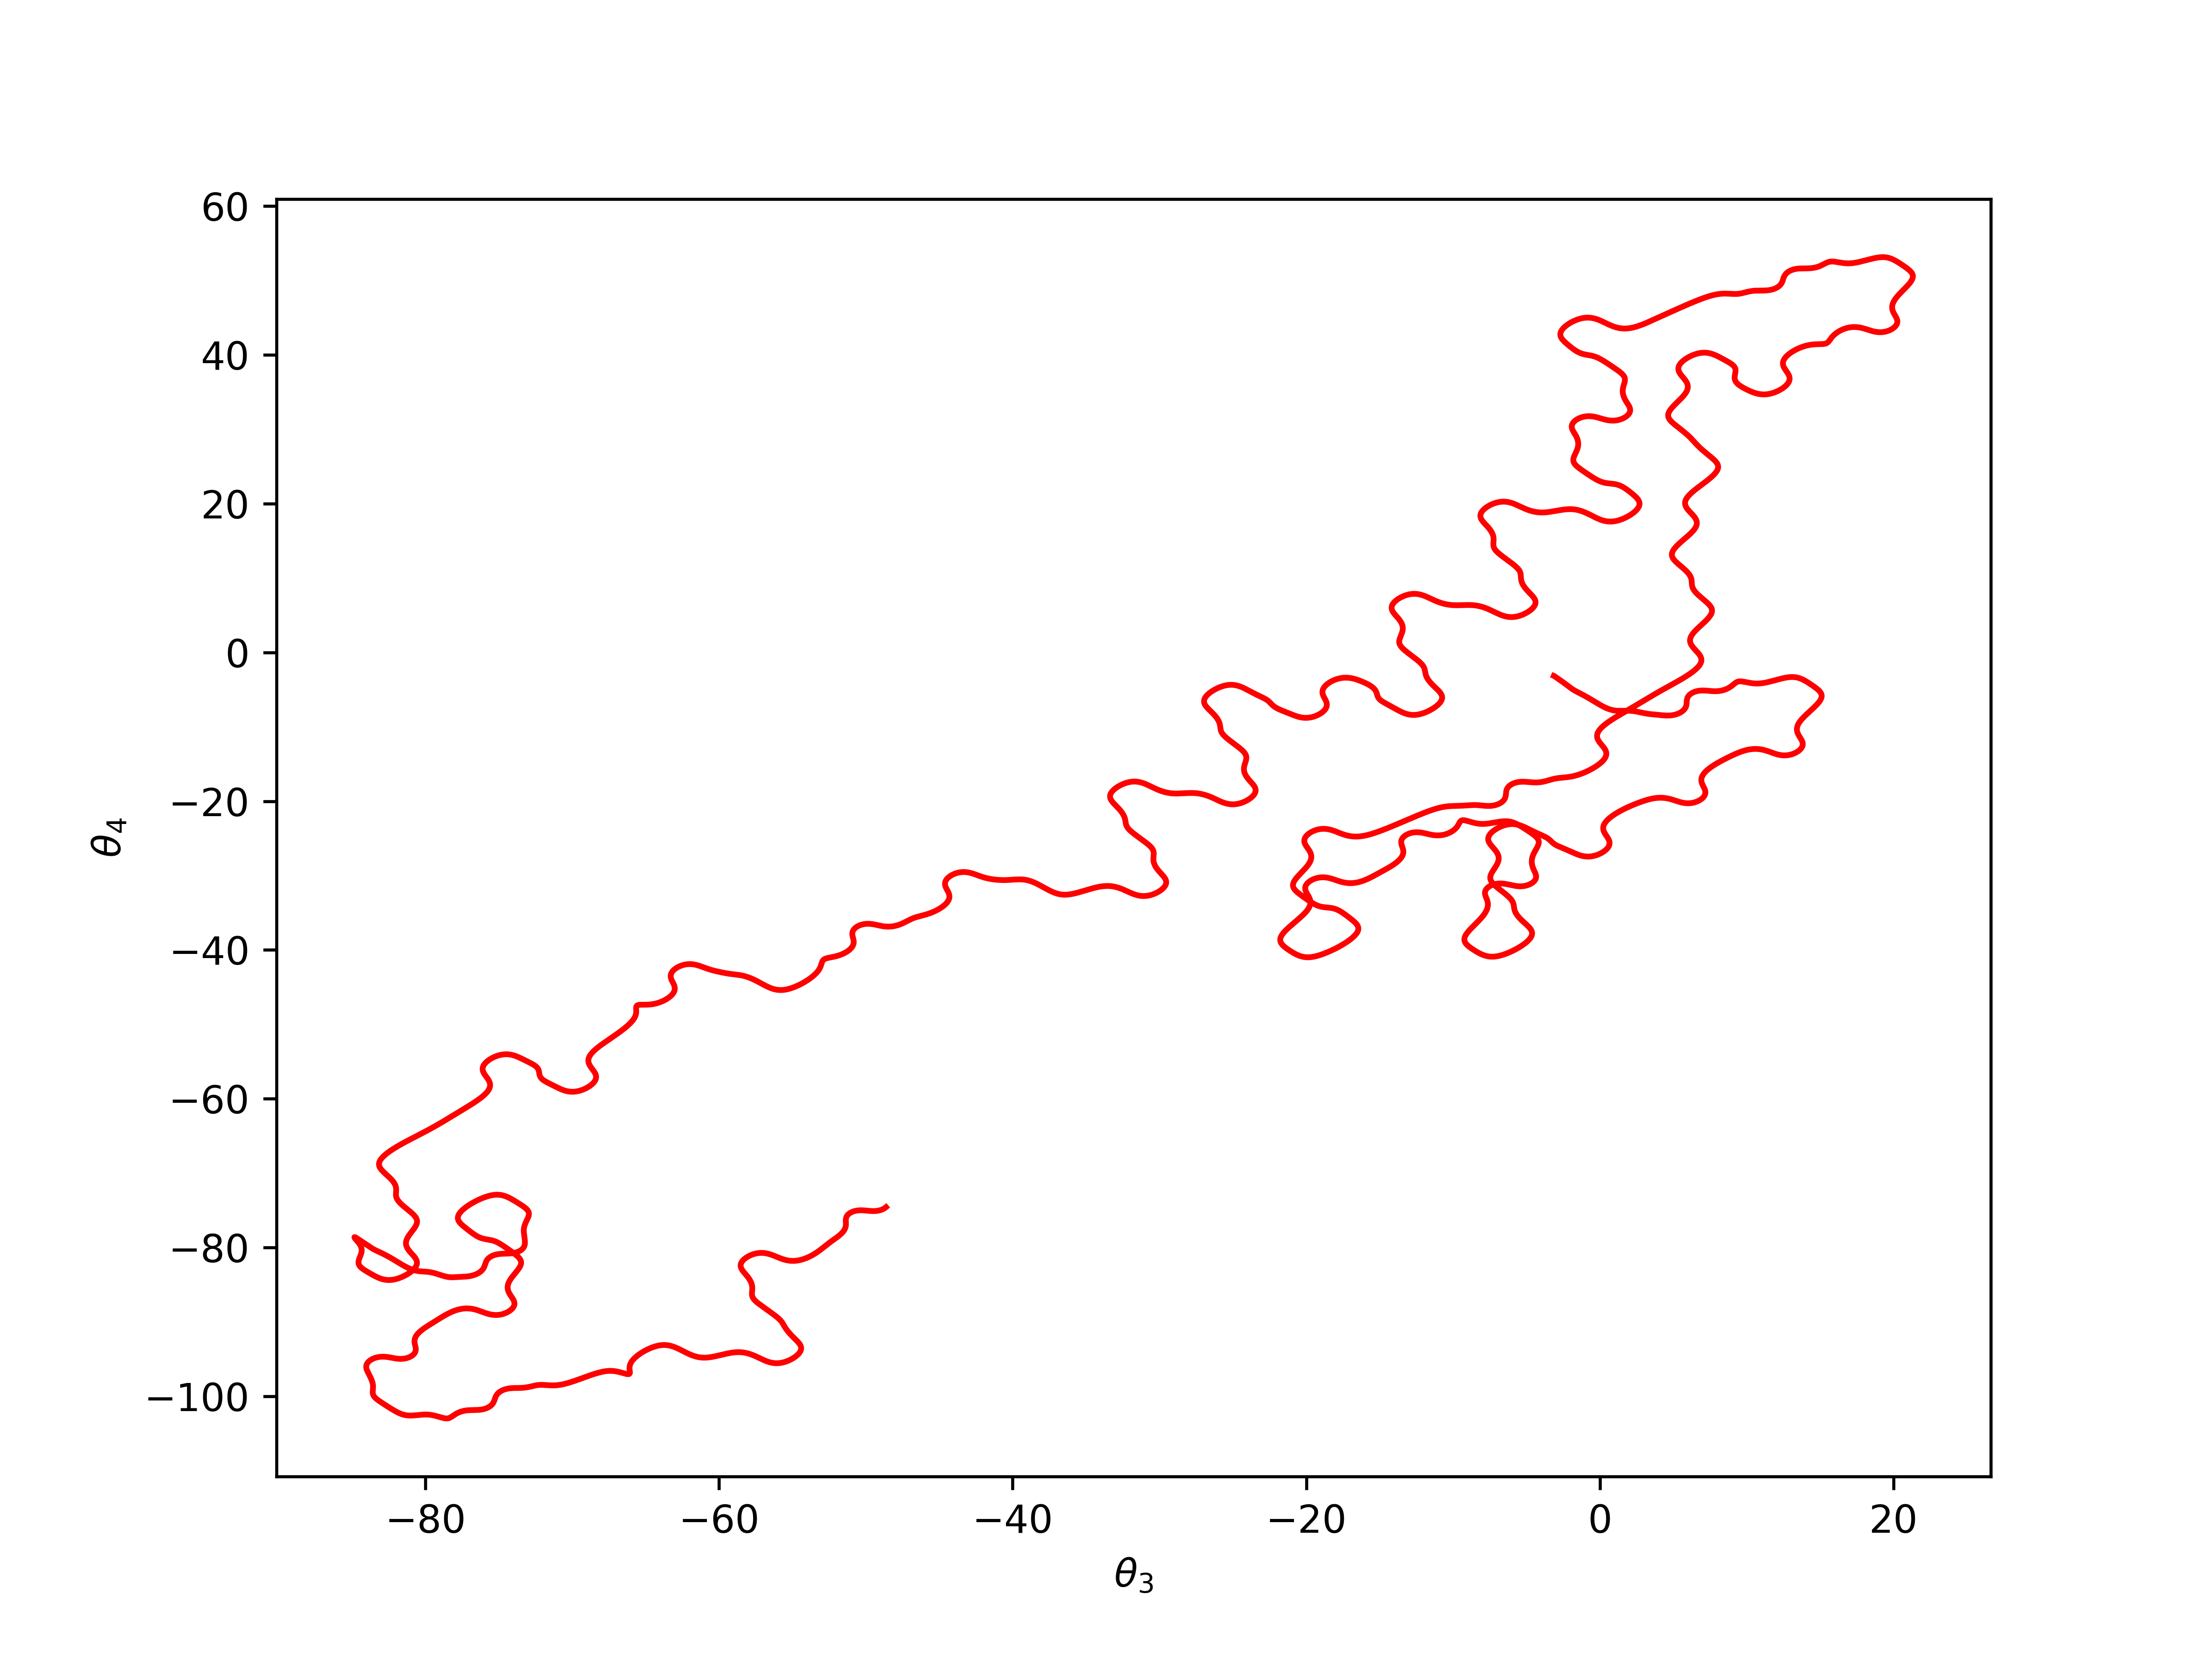
\includegraphics[width=\linewidth]{img/theta_theta_2.png}
  \caption{Pendulum 2 $\theta_3$ vs $\theta_4$.}\label{fig:theta_vs_theta_2}
\endminipage\hfill
\minipage{0.32\textwidth}%
  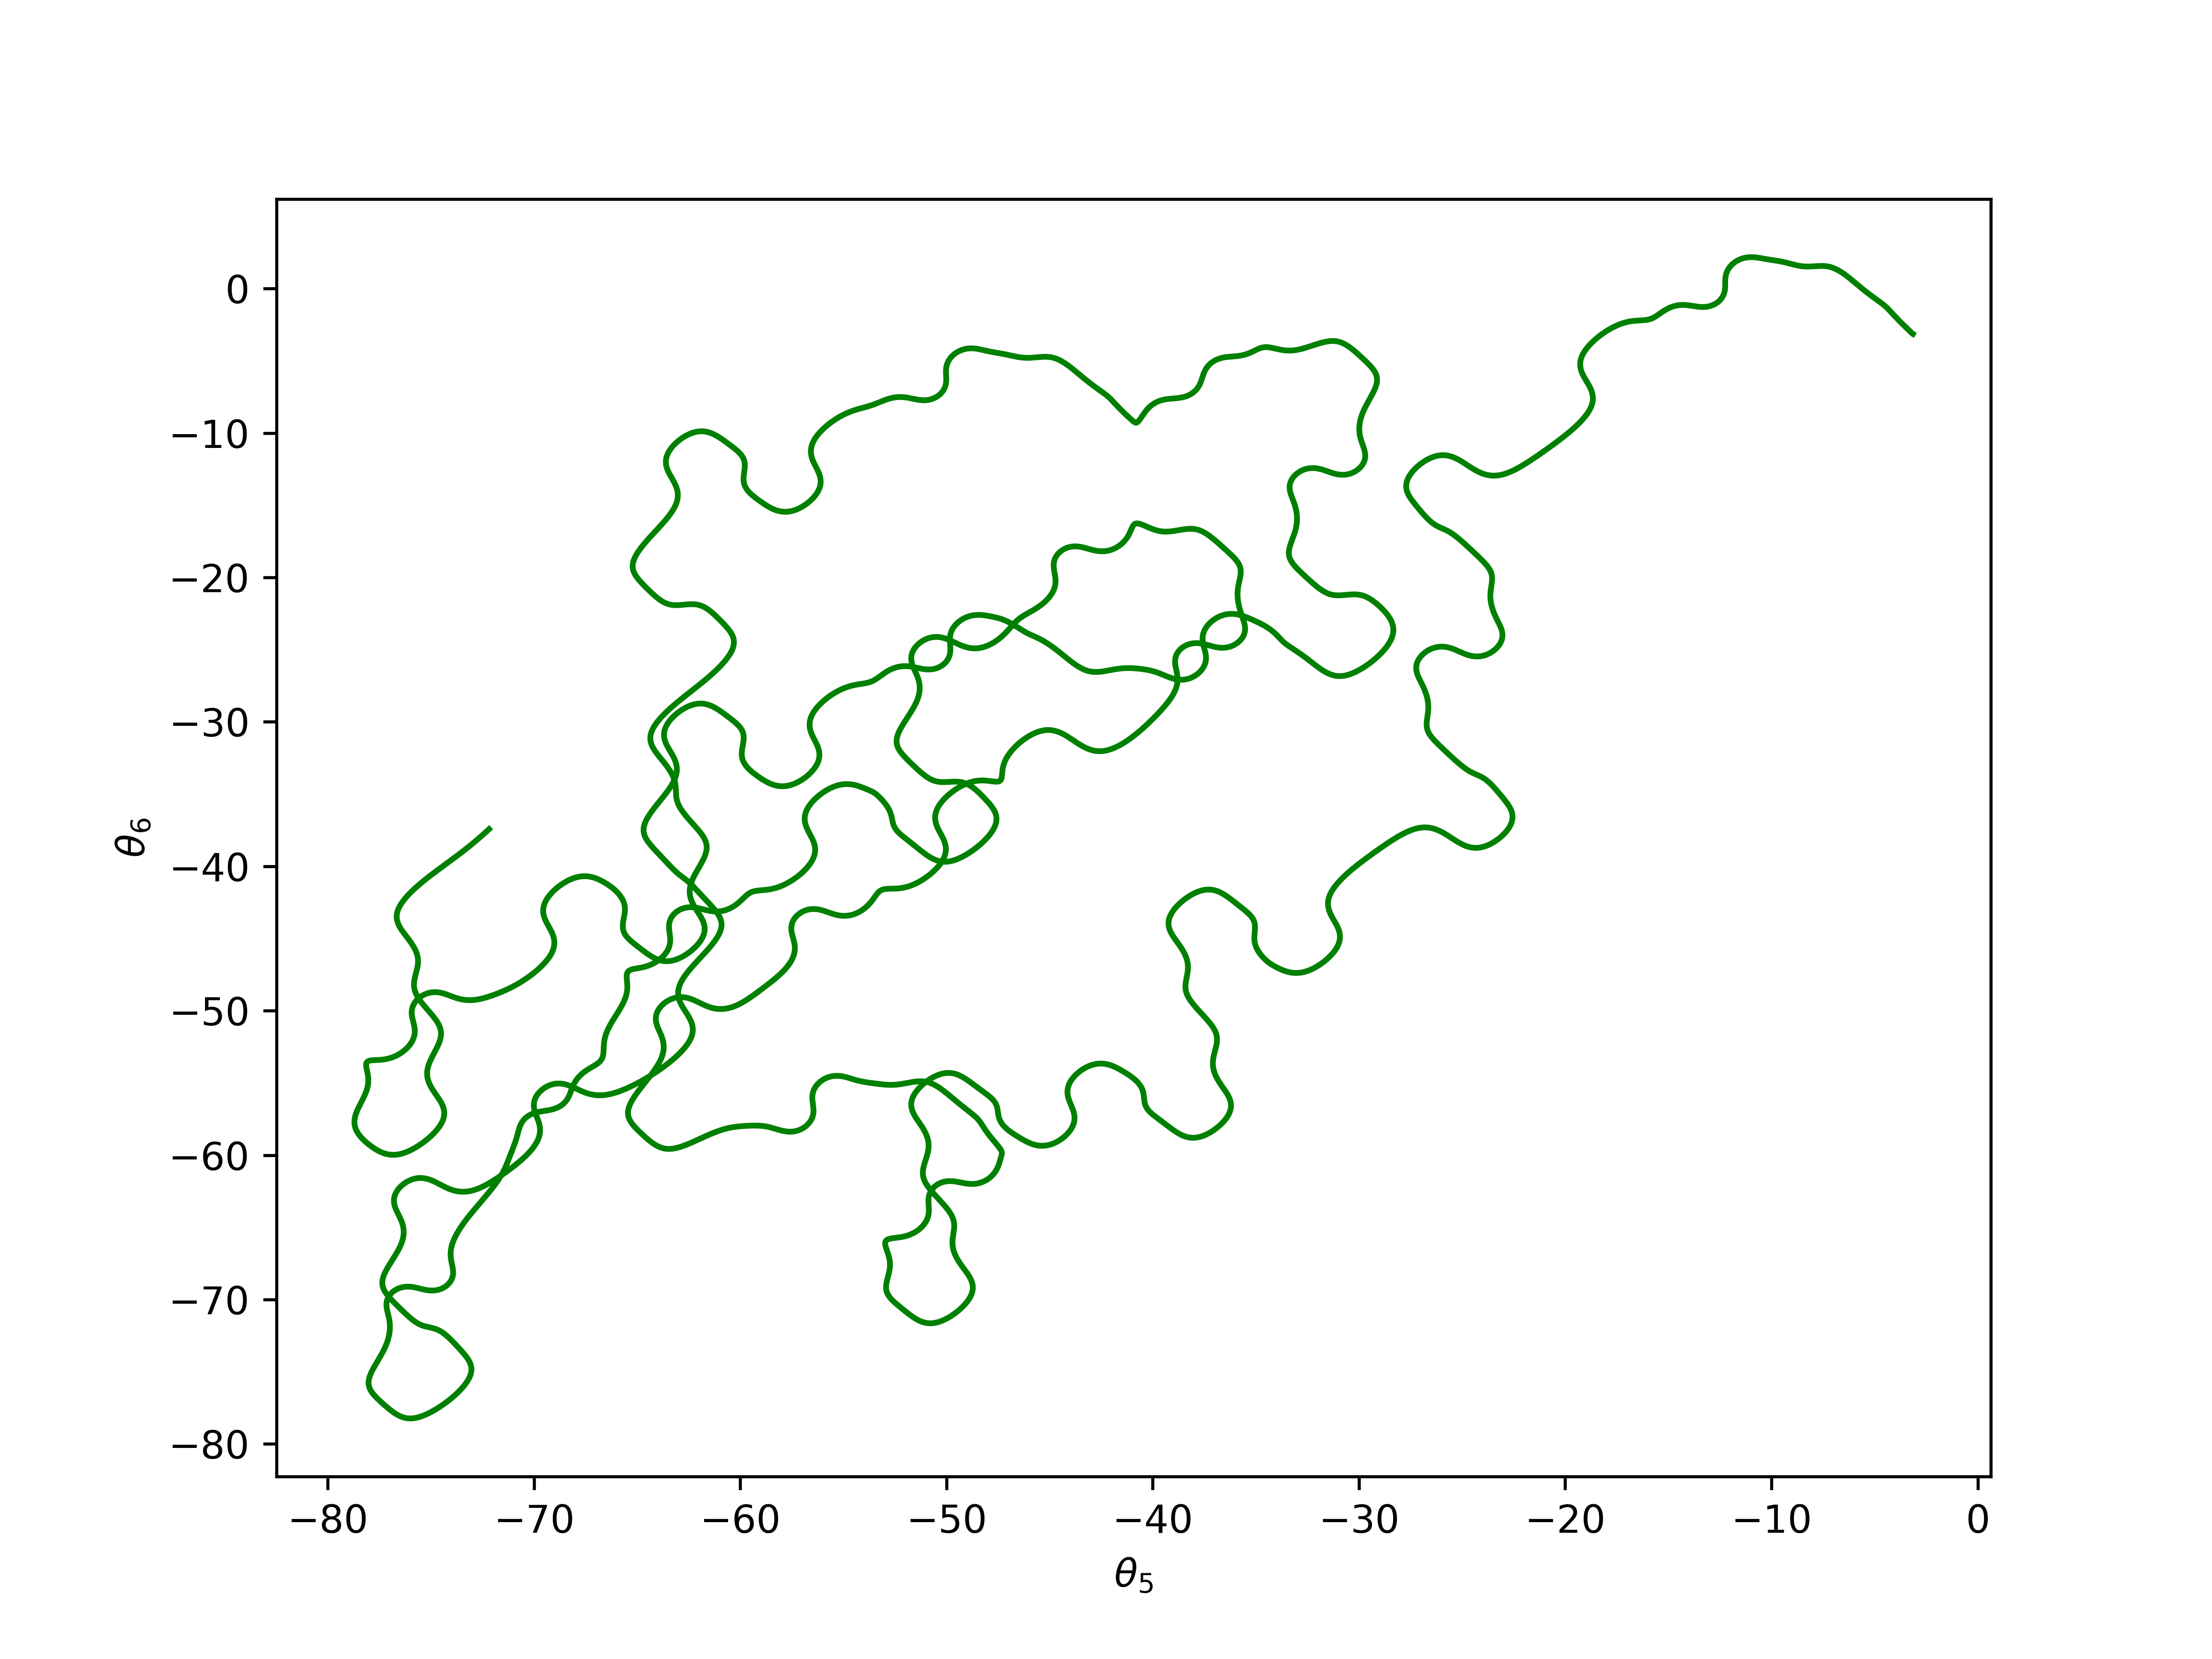
\includegraphics[width=\linewidth]{img/theta_theta_3.png}
  \caption{Pendulum 3 $\theta_5$ vs $\theta_6$.}\label{fig:theta_vs_theta_3}
\endminipage
\end{figure}

The Figure above, just like the figure below, shows how much a system can vary just base on the initial conditions. What the figure above also shows is that we also lose the pattern the the near perfect harmonic motion gave us for the theta vs theta plot. Instead, this plot becomes very chaotic and there is no pattern since the theta values can rapidly change in value. 


\begin{figure}[h]
    \centering
    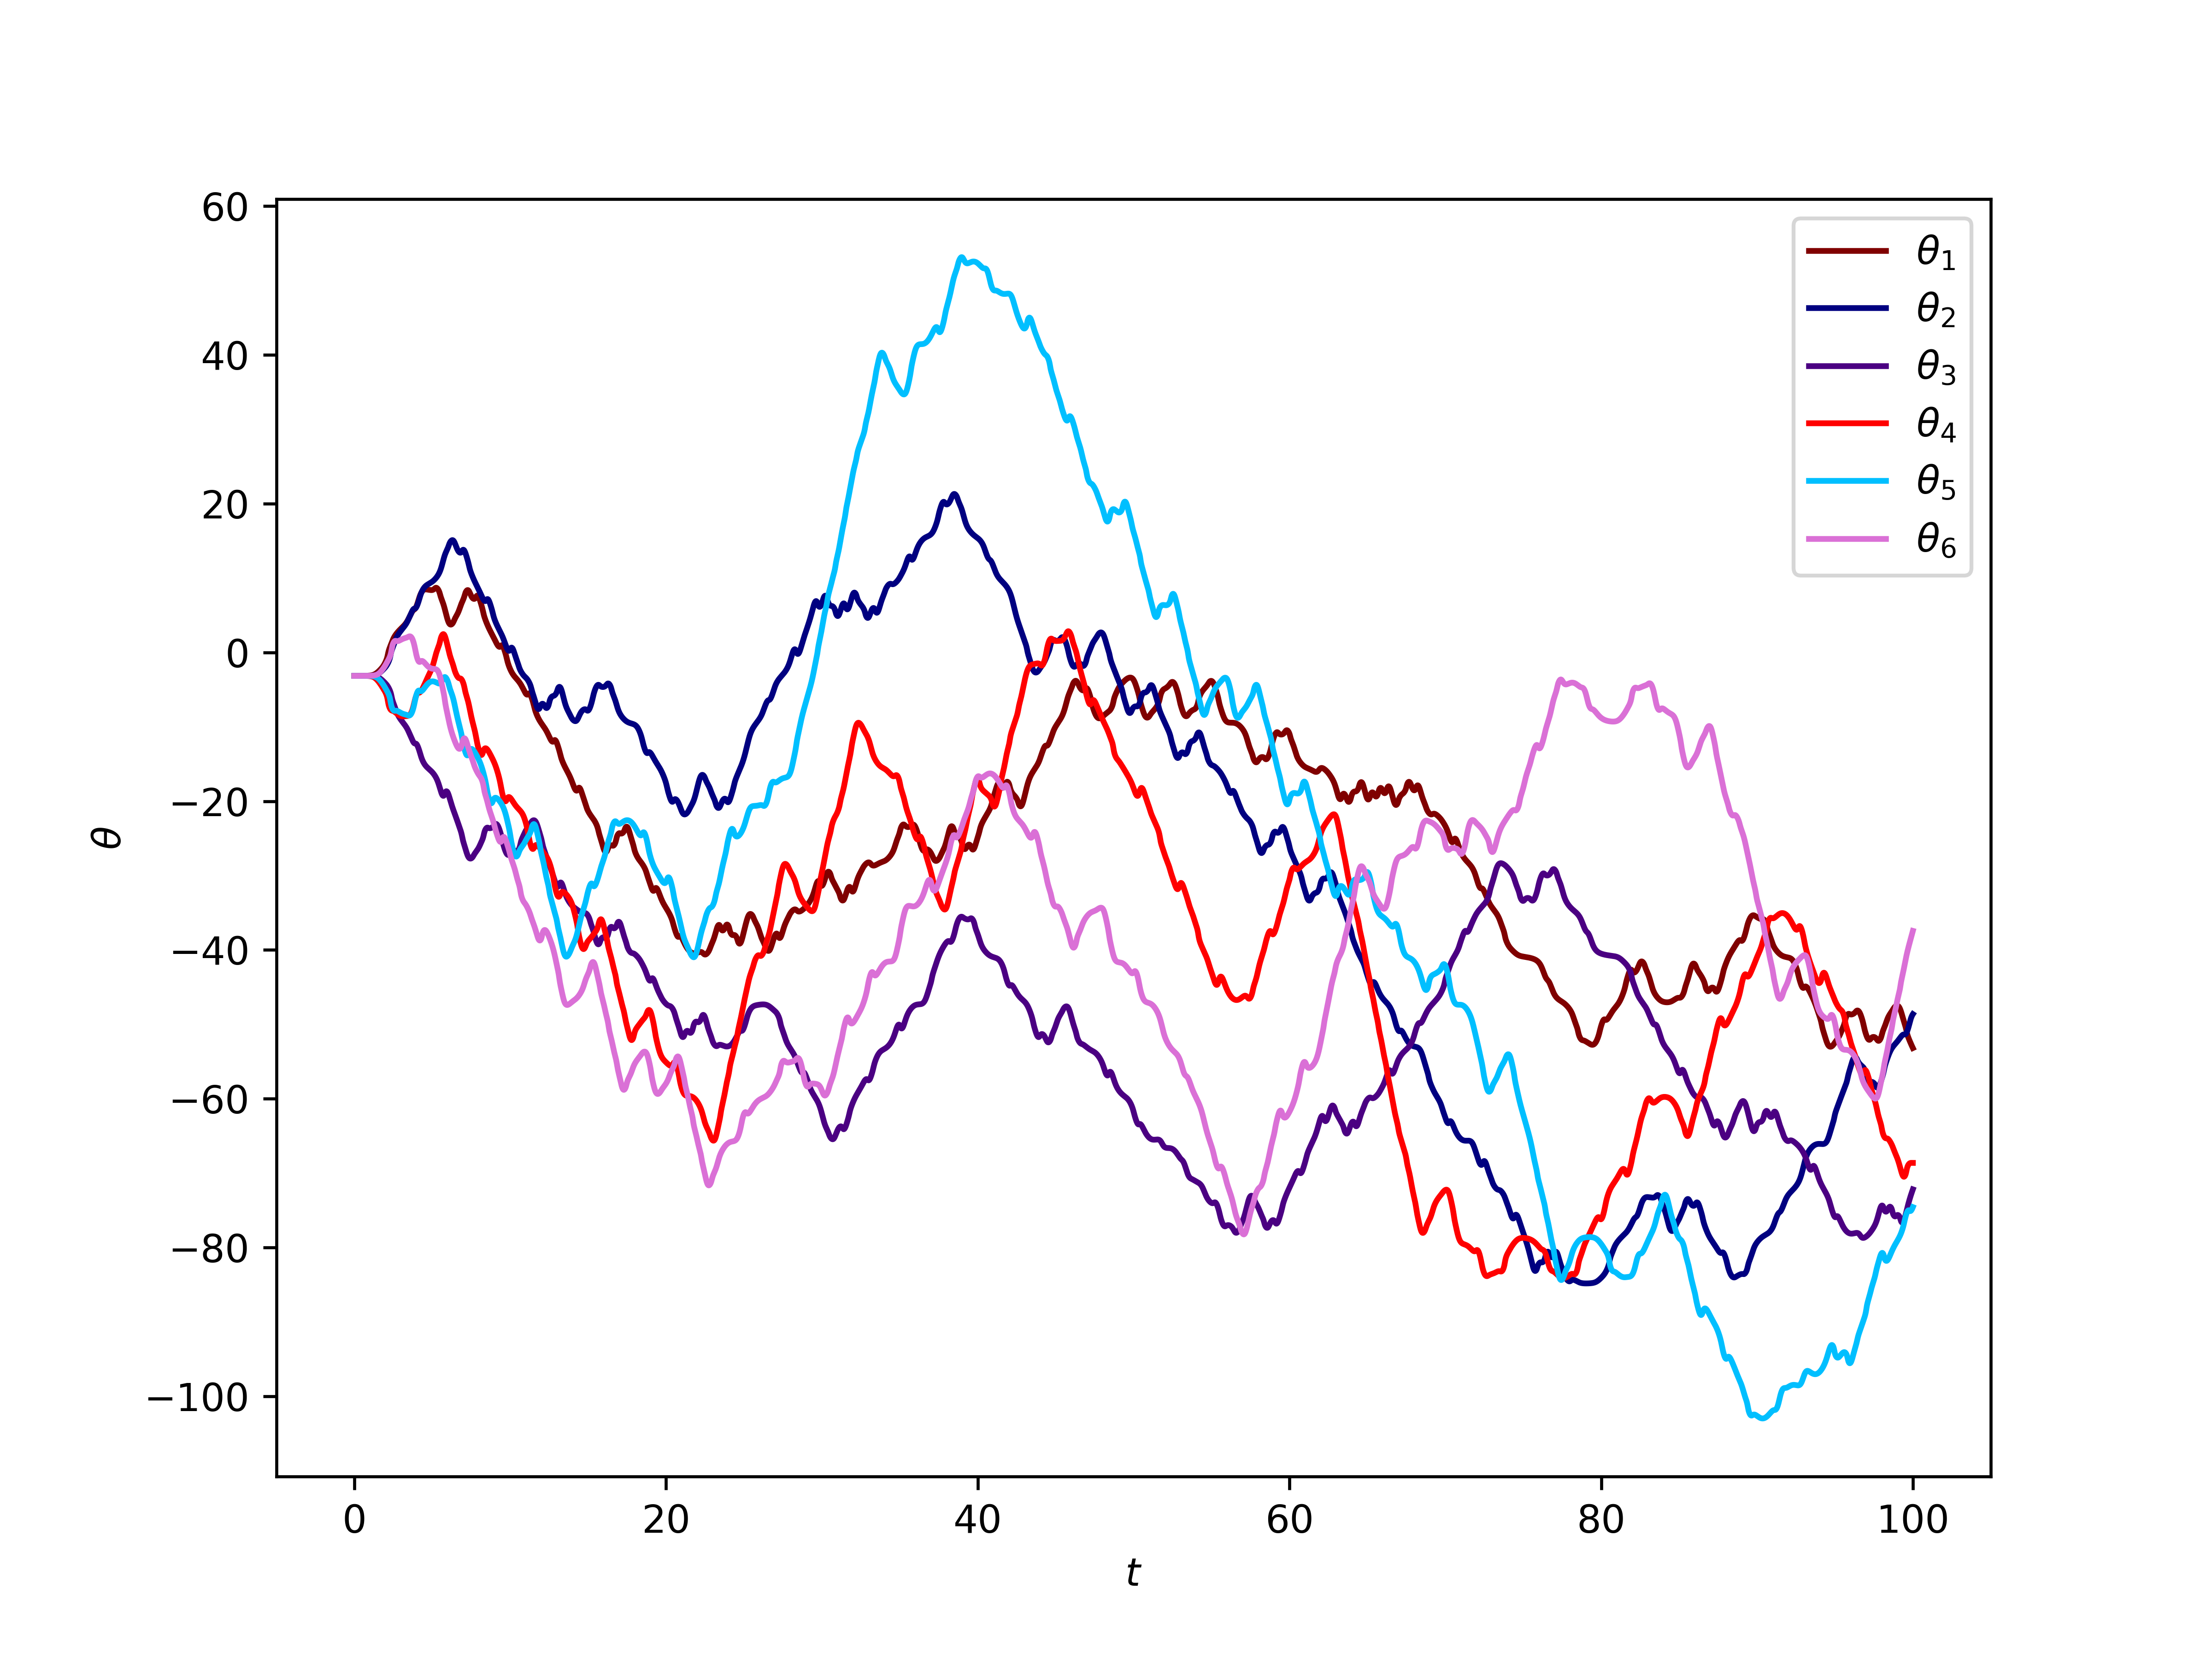
\includegraphics[width=0.75\textwidth]{img/compare_double_pen_1.png}
    \caption{Three different double pendulum systems where initial values vary by 0.001 from each other.}
    \label{fig:compare_theta_vs_time}
\end{figure}
 
As you can see in the figure above, each $\theta$ angle differs by a large amount, even though the initial conditions for the three different double pendulum systems only varied by 0.001 from each system. This image also has a great demonstration on just how different a system can turn out by a slight variation in how the system is made to start out.


\section{Conclusion}

From pen and paper to computer script Lagrangian mechanics are simple to model. Most of the work in the model process involved finding the Lagrangian and the equation(s) of motion. Once these are found, working backwards from the initial step help allow us to computationally model the Lagrange mechanics method. Modeling a Lagrangian can give us good incite to how a system behaves. It allows for stress testing and breaking the system all together by finding unstable conditions. This process above allow show how complex a system can get with minor variations and aloows for a quick analysis of system. This proves that its a quick and simple solution to find a lot about a system in a relatively short amount of time.

\clearpage{}



\clearpage{}
%
% ---- Bibliography ----
%
% BibTeX users should specify bibliography style 'splncs04'.
% References will then be sorted and formatted in the correct style.
%

% Find from the left the folder bibliography/ and locate first.bib. you
% can generate your bibtex references using citethisforme and paste it inside the first.bib file
% to cite a bibliography, use \cite{bisht_hinrichs_skrupsky_venkatakrishnan_2014} (example)
% those are citations embedded to texts
% please check out https://www.latex-tutorial.com/tutorials/bibtex/

\bibliography{bibliography/first}
\bibliographystyle{splncs04}

[1] Levien, R. & Tan, Sze. (1993). Double pendulum: An experiment in chaos. American Journal of Physics - AMER J PHYS. 61. 1038-1044. 10.1119/1.17335. 

[2] Mukul K. Gupta, Kamal Bansal, Arun K. Singh,
Mass and Length Dependent Chaotic Behavior of a Double Pendulum,
IFAC Proceedings Volumes, Volume 47, Issue 1, 2014

[3] Troy Shinbrot, Celso Grebogi, Jack Wisdom, James Yorke.  Chaos in a double pendulum.  Amer-ican  Journal  of  Physics,  American  Association  of  Physics  Teachers,  1992,  60,  pp.491  -  491.￿10.1119/1.16860￿.



%Appen

\section*{Appendix}

The source code for this project can be found here at \\
https://github.com/timothypholmes/lagrangian-mechanics

\end{document}